\chapter{Grundlagen}\label{chapter:Grundlagen}
In diesem Kapitel wird erläutert, was der Begriff \frqq Industrie 4.0\flqq\  bedeutet, vor welche Herausforderungen sie uns stellt und welche Effekte mit ihr einhergehen. Des Weiteren behandelt dieses Kapitel grundlegende Sachverhalte bezüglich Fertigungsrobotern und dem hier als Substitution benutzten  \textit{Lego Mindstorms EV3} sowie Grundlagen zu AR und der genutzten Brille \textit{Microsoft HoloLens}.
\section{Industrie 4.0}\label{sec:i40}
Eine \frqq Industrielle Revolution\flqq\ bezeichnet \frqq einen raschen Wandel von Produktionstechniken und, daraus abgeleitet, von wirtschaftlich-gesellschaftlichen Strukturen.\flqq\footnote{ Prof. Dr. Voigt, 2016, [Accessed: 06.01.2017].} Die \frqq Industrie 4.0\flqq\ bezeichnet das Ergebnis der vierten \textit{Industriellen Revolution}. Sie reiht sich an der Spitze von drei Vorgängern ein:
\begin{itemize}
	\item Die erste \textit{Industrielle Revolution}, etwa um 1750, bei der Arbeits- und Kraftmaschinen die Industrialisierung und das Verhindern von Hungerkatastrophen ermöglichte.
	\item Die zweite \textit{Industrielle Revolution}, etwa um 1870, die Wohlstand durch arbeitsteilige Massenproduktion mit Hilfe elektrischer Energie schaffte.
	\item Und die dritte \textit{Industrielle Revolution}, seit circa 1960, welche durch Elektronik und IT automatisierungsgetriebene Rationalisierung sowie die variantenreiche Serienproduktion ermöglichte.\footnote{ Vgl. Dipl.-Ing. Jäger et al, 2015.}
\end{itemize}
Diese Entwicklung ist zusätzlich schematisch in Abbildung~\ref{fig:VerlaufIndustrie402} dargestellt.
\begin{figure}[ht]
	\centering
	\includegraphics[width=.8\textwidth]{figuren/Industrie-40-Definition-Stufen-Revolution-01}
	\caption{Verlauf Industrieller Revolutionen ab 1800 bis heute. Bildquelle: \cite{i40Verlauf}.}
	\label{fig:VerlaufIndustrie402}
\end{figure}
Der Begriff \frqq Industrie 4.0\flqq\ ist ursprünglich ein Projektname einer Arbeitsgruppe des Bundesministerium für Wirtschaft und Energie (BMWi). Es sind zahlreiche Beschreibungen zu finden, die sich sehr stark ähneln. Für die folgende Arbeit wird daher die Definition des BMWi beibehalten:
\begin{quote}
	\frqq In der Industrie 4.0 verzahnt sich die Produktion mit modernster Informations- und Kommunikationstechnik [...] (zu)
	%. Treibende Kraft dieser Entwicklung ist die rasant zunehmende Digitalisierung von Wirtschaft und Gesellschaft. Sie verändert nachhaltig die Art und Weise, wie zukünftig in Deutschland produziert und gearbeitet wird: Nach Dampfmaschine, Fließband, Elektronik und IT bestimmen nun 
	intelligente(n) Fabriken (sogenannte „Smart Factories“) [...]
	%die vierte industrielle Revolution. Technische Grundlage hierfür sind intelligente, digital vernetzte Systeme, mit deren Hilfe eine weitestgehend selbstorganisierte Produktion möglich wird: 
	Menschen, Maschinen, Anlagen, Logistik und Produkte kommunizieren und kooperieren in der Industrie 4.0 direkt miteinander. Produktions- und Logistikprozesse zwischen Unternehmen im selben Produktionsprozess werden intelligent miteinander verzahnt, um die Produktion noch effizienter und flexibler zu gestalten.
	
	So können intelligente Wertschöpfungsketten entstehen, die zudem alle Phasen des Lebenszyklus des Produktes miteinschließen -- von der Idee eines Produkts über die Entwicklung, Fertigung, Nutzung und Wartung bisn hin zum Recycling. [...] %Auf diese Weise können zum einen Kundenwünsche von der Produktidee bis hin zum Recycling einschließlich der damit verbundenen Dienstleistungen mitgedacht werden. Deshalb können Unternehmen leichter als bisher maßgeschneiderte Produkte nach individuellen Kundenwünschen produzieren. Die individuelle Fertigung und Wartung der Produkte könnte der neue Standard werden. Zum anderen können trotz individualisierter Produktion die Kosten der Produktion gesenkt werden.Durch die Vernetzung der Unternehmen der Wertschöpfungskette ist es möglich, nicht mehr nur einen Produktionsschritt, sondern die ganze Wertschöpfungskette zu optimieren. Wenn alle Informationen in Echtzeit verfügbar sind, kann ein Unternehmen z.B. frühzeitig auf die Verfügbarkeit bestimmter Rohstoffe reagieren [...] (und) Produktionsprozesse können unternehmensübergreifend so gesteuert werden, dass sie Ressourcen und Energie sparen.
	[...]\flqq\footnote{ BMWi, Hrsg., 2016, [Accessed: 06.01.2017].}
	%	URL: \url{http://www.plattform-i40.de/I40/Navigation/DE/Industrie40/WasIndustrie40/was-ist-industrie-40.html}.}
	%
	%	Insgesamt kann die Wirtschaftlichkeit der Produktion gesteigert, die Wettbewerbsfähigkeit der Industrie in Deutschland gestärkt und die Flexibilität der Produktion erhöht werden.
\end{quote}
Momentan eher als Marketingbegriff benutzt, fasst der Ausdruck \frqq Industrie 4.0\flqq\ sehr gut zusammen, wie die Produktion in Deutschland, aber auch weltweit, in Zukunft aussehen kann. Ein hochgerechnetes Investitionsvolumen von jährlich 40 Mrd. Euro in den nächsten fünf Jahren zeigt deutlich, dass vernetzte und intelligente Produktionsstätten ein Hauptanliegen der deutschen Industrie und Wirtschaft darstellen\footnote{ Vgl. Dr. Geissbauer / Schrauf / Koch / et al. (2016), S.7.}. Sie sind maßgeblich dafür verantwortlich, dass Deutschland seine Vorreiterrolle und sein Ansehen als Motor moderner, effizienter und qualitativ hochwertiger Industrieanlagen weltweit behaupten und weiter ausbauen kann.

%vgl. PricewaterhouseCoopers Aktiengesellschaft Wirtschaftsprüfungsgesellschaft, Dr. Geissbauer / Schrauf / Koch / et al, S.7, 2016}
%Marktforschungsunternehmens PriceWaterhouseCooper (PwC) und die des Fraunhofer-Institut für Produktionsanlagen und Konstruktionstechnik (IPK) gewählt: \glqq 
%\footnote{(PwC (Hrsg.), 2016, S.1)}
\subsection{Herausforderungen}\label{ssec:i40Challenges}
Deutschland ist, wie in Abbildung \ref{fig:EULabourPerHour} zu sehen, ein Hochlohnstandort. Eine maßgebliche Herausforderung ist daher: Die Produktion durch Innovationen profitabel im Inland zu betreiben, statt sie ins Ausland zu verlagern.

\begin{figure}[ht]
	\centering
	\includegraphics[width=1.\textwidth]{figuren/Estimated_hourly_labour_costs_2015}
	\caption{Durchschnittliche Arbeitskosten pro Stunde in Europa, 2015. Bildquelle: \cite{hochlohnstandort}.}
	\label{fig:EULabourPerHour}
\end{figure}

Des Weiteren zählt die Bundesrepublik Deutschland zu einem der Länder, dessen Rohstoffverlangen bei weitem die Menge dessen übersteigt, welche im Inland abgebaut werden kann. Es bilden sich Abhängigkeiten, um die Rohstoffversorgung zu sichern. Beispielsweise importierte die Bundesrepublik im Jahr 2005 Waren mit dem Gesamtwert von 625 Mrd. Euro, darunter 26,5 Mio. Tonnen Steinkohle und 110 Mio. Tonnen Rohöl.\footnote{ Topel / Seibel, Hrsg., o. J., [Accessed: 11.01.2017].}
Um wettbewerbsfähig und unabhängig zu sein, müssen die Produktionsstätten der Zukunft ressourcensparend und vor allem energieeffizient produzieren.
Hierzu gesellt sich auch das Schlagwort \frqq Urbane Produktion\flqq. Es bedeutet: \glqq das Umfeld einer Produktionsstätte in den Bilanzierungsrahmen der energetischen Optimierung einzubeziehen\grqq.\footnote{ Fraunhofer-Institut für Produktionstechnik und Automatisierung, Hrsg., o.J., [Accessed: 11.01.2017].} Dazu zählen sowohl Recycling als auch Abwärme und andere passive Rohstoffe.

Außerdem sehen sich Gesellschaften, die ein gewisses Maß an Wohlstand erreicht haben, mit einem demographischen Wandel konfrontiert.\footnote{ Vgl. Roser / Ortiz-Ospina, 2017, [Accessed: 01.02.2017].}
\begin{figure}[ht]
	\centering
	\includegraphics[width=1.\textwidth]{figuren/SOZ_01_04_Bevoelkerungsentwicklung_und_Altersstruktur}
	\caption{Bevölkerungsentwicklung in Deutschland von 1950-2050. Bildquelle: \cite{demographischerWandel}.}
	\label{fig:DEDemographischerWandel}
\end{figure}
In Abbildung~\ref{fig:DEDemographischerWandel} ist die Bevölkerungsentwicklung in Deutschland von 1950 bis 2050 zu sehen. Abzuleiten daraus ist, dass der Anteil der Bevölkerung im arbeitsfähigen Alter kleiner, und der nicht arbeitsfähige Anteil\footnote{ Vgl. Statistisches Bundesamt, Bevölkerung nach Altersgruppen, Hrsg., [Accessed: 11.01.2017].} größer wird. Dieser Wandel spannt verschiedene Problemfelder auf, deren Lösung von verschiedenen Seiten gefordert wird. Welche Lösungsansätze durch die \frqq4. Industrielle Revolution\flqq\ entstehen, wird im Folgenden erläutert.
\subsection{Effekte}\label{ssec:i40Effects}
Die aus den Herausforderungen resultierenden Effekte versucht die \frqq Industrie 4.0\flqq\ bewusst zu adressieren und anzugehen.
Intelligente Fabriken können das Arbeiten am Hochlohnstandort wieder profitabel machen. Das BMWi beschreibt diesen Wandel wie folgt: \glqq Industrie 4.0 bedeutet gute Arbeit, nicht menschenleere Fabriken. Vielmehr verändert sich das Arbeiten: Die Beschäftigten müssen stärker in die Prozesse eingebunden werden, zum Bespiel[sic] um Abläufe zu koordinieren, die Kommunikation zu steuern und eigenverantwortlich schnell Entscheidungen zu treffen\grqq.\footnote{ BMWi, Hrsg., 2016, [Accessed: 09.01.2017].}

Verzahnung von industrieller Produktion mit modernster Informations- und Kommunikationstechnik soll in hoher Individualität, Effizienz und Kostenersparnis münden. Schon heute ermöglichen Innovationen, wie beispielsweise ein intelligenter Handschuh\footnote{ Handschuh der beispielsweise Produktions- und Logistikprozesse verbessert und vereinfacht.}, Zeitersparnisse und mehr Effizienz im Logistiksektor. Eine \textit{Wearable}-Lösung wie diese begleitet einen Arbeiter auf dem Weg in die \frqq Industrie 4.0\flqq, ist jedoch eher in Logistik- und Zuliefererbetrieben anzusiedeln. Allerdings soll in Zukunft die Produktion durch \textit{Cyber Physical Systems}\footnote{ Cyber-Physische Systeme (CPS) sind Systeme mit eingebetteter Software und Elektronik, die über Sensoren und sogenannte Aktoren (Antriebselemente) mit der Außenwelt verbunden sind.} digitalisiert werden, damit dabei eine smarte Wertschöpfungskette entsteht, die ihren Energie- und Ressourcenbedarf optimal regulieren und ausschöpfen kann. Hinzukommend könnten Kreisläufe entstehen, die urbane Gegebenheiten, von Abwärme bis hin zu Recycling mit berücksichtigen und so die Produktionsprozesse noch umweltfreundlicher und effizienter gestalten.

Die Herausforderung einer alternden Gesellschaft bedeutet den Verlust von Arbeitskraft in menschlicher Form. Eine Industrielandschaft, in der Maschinen den Hauptteil der zu bewerkstelligenden Aufgaben erledigen können und nur ein vergleichsweise kleiner Teil der Gesellschaft durch fachliche Kompetenz diese Maschinen entwickeln und warten muss, kann einen solchen Wandel ausgleichen.

Diese Effekte durch gezielte Investitionen und Entwicklungen im Fachbereich der Sensorik und Robotik anzugehen, ist das Hauptanliegen der \frqq Industrie 4.0\flqq.\newpage
\section{Robotik}\label{sec:robots}
Die interdisziplinäre Kategorie der Robotik bezeichnet ein Teilgebiet des Ingenieurwesens, welches sich aus den Hauptbestandteilen Maschinenbau, Elektrotechnik und Informatik zusammensetzt und dessen Wortursprung im slawischen Wort \frqq robota\flqq\ liegt und soviel bedeutet wie \frqq Arbeiten\flqq.\footnote{ Vgl. Siciliano / Khatib, S.1, 2008.} 1920 wurde der Begriff vom tschechischen Schriftsteller Karel Čapeks in seinem Schauspiel \frqq R. U. R.\flqq\ (Rossums Universal-Roboter) im Sinne eines Maschinenmenschen erwähnt und dadurch geprägt. Die Robotik ist eine der Leitindustrien des 21. Jahrhunderts, woraus eine enge Verbindung zur Mensch-Maschine-Interaktion, Psychologie, Soziologie (soziale Robotik) und Philosophie (Maschinenethik) entsteht.\footnote{ Vgl. Prof. Dr. Bendel, Wirtschaftslexikon Stichwort: Robotik, o.J., o.S.}
\subsection{Überblick, Entwicklung und Forschungsstand}\label{ssec:researchRobots}
Der Verband Deutscher Ingenieure (VDI) definiert in seiner \textit{Richtlinie 2860} Roboter wie folgt: \frqq Industrieroboter sind universell einsetzbare Bewegungsautomaten mit mehreren Achsen, deren Bewegungen hinsichtlich Bewegungsfolge und Wegen bzw. Winkeln frei (d.h. ohne mechanischen bzw. menschlichen Eingriff) programmierbar und gegebenenfalls sensorgeführt sind. Sie sind mit Greifern, Werkzeugen oder anderen Fertigungsmitteln ausrüstbar und können Handhabungs- und/oder Fertigungsaufgaben ausführen\flqq.\footnote{ VDI-Richtlinie 2860, Blatt 1.}

Angefangen mit Heron von Alexandria (Abb. \ref{fig:Automata}) und seinen Entwürfen für ein Automatentheater um etwa 100 nach Christus, über die drei Droiden (Zeichner, Schriftsteller und Klavierspieler) aus Abbildung \ref{fig:jaquet}, gebaut 1774 von Jaquet Droz und dessen Sohn, bis zur Erfindung des Industrieroboters durch George Devol 1954 (Patentzeichnung in Abbildung \ref{fig:Devol_Patent}) sind Automaten dafür erdacht worden, den Menschen Arbeiten abzunehmen und sie durch die Automatisierung von Arbeitsschritten zu entlasten.\footnote{ Vgl. Prof. Dr.-Ing. Linemann, S.4 ff., 2016.}
\begin{figure}[H]
	\centering
	\includegraphics[width=0.5\textwidth]{figuren/Hero_of_Alexandria_Automata}
	\caption{Skizze von Heron von Alexandria \frqq Automata\flqq. Bildquelle: \cite{automata}.}
	\label{fig:Automata}
\end{figure}
\begin{figure}[H]
	\centering
	\includegraphics[width=1.\textwidth]{figuren/Jaquet}
	\caption{Die Droiden von Jaquet Droz und seinem Sohn: Der Zeichner (links) und seine Zeichnung (links unten), Der Schreiber (mitte) und dessen Text (rechts unten) und die Musikerin (rechts). Bildquelle: \cite{zeichner}, \cite{schreiber}, \cite{musikerin}, \cite{zeichnung}, \cite{text}.}
	\label{fig:jaquet}
\end{figure} 
\begin{figure}[H]
	\centering
	\includegraphics[width=.5\textwidth]{figuren/Devol_Patent_1954}
	\caption{Patentzeichnung für den ersten Industrieroboter. Bildquelle: \cite{devol}.}
	\label{fig:Devol_Patent}
\end{figure}
Laut der oben genannten VDI-Richtlinie sind Industrieroboter eine Untergruppe der Handhabungsgeräte. Abbildung \ref{fig:Handhabungsgeräte} zeigt dabei ihre Unterteilung in verschiedene Untergruppen. Zu erwähnen ist, dass die Kategorien \frqq Manipulator, Teleoperator\flqq\ und \frqq Industrieroboter\flqq\ in Zukunft wieder zusammengeführt werden könnten. So zählt auch in dieser Abschlussarbeit die prototypische Implementierung mehr zur Kategorie der Teleoperator. Allerdings wird darauf hingewiesen, dass Industrieroboter durch das verschmelzen der Arbeitsbereiche von Mensch und Maschine immer mehr zu \frqq Cobots\flqq\footnote{ Kooperierende Roboter (Cobot), bezeichnen Roboter die gemeinsam
	mit Menschen Arbeit verrichten.} werden könnten und somit ein hybrides Dasein zwischen Werkzeug und autonomer Maschine pflegen könnten.

\begin{figure}[H]
	\centering
	\includegraphics[width=.5\textwidth]{figuren/Handhabungsgeraete}
	\caption{Unterteilung von Handhabungsgeräten in Untergruppen. Bildquelle: \cite{pdf:roboticScript}.}
	\label{fig:Handhabungsgeräte}
\end{figure}
Man unterscheidet vier Hauptgruppen von Robotern:
\begin{itemize}
	\item Industrieroboter
	\item Serviceroboter
	\item Geländeroboter
	\item Autonome Roboter / Agentensysteme
\end{itemize}
Betrachtet man die Gruppe der Industrieroboter genauer, ist es wichtig sich über die genaue Beschaffenheit des Roboters im Klaren zu sein, da sie sowohl seinen Arbeitsraum als auch die Komplexität seiner Bewegungen definieren. Die Hauptkomponenten sind, wie in Abbildung \ref{fig:Roboter_Beschaffenheit} gezeigt, das Fahrzeug, welches die Lokomotion bestimmt, der Roboterarm, der den Endeffektor führt, und der Endeffektor selbst, welcher mit der Umwelt interagiert.
\begin{figure}[H]
	\centering
	\includegraphics[width=.5\textwidth]{figuren/Roboter_Beschaffenheit}
	\caption{Schematische Darstellung eines Industrieroboters. Bildquelle: \cite{pdf:roboticScript}.}
	\label{fig:Roboter_Beschaffenheit}
\end{figure}
Alle genannten Komponenten haben Freiheitsgrade, welche die Komplexität der Dynamik und Kinematik des Roboters festlegen. Die folgende Formel bestimmt dabei die Bewegungsfreiheitsgrade eines Roboters:
\begin{equation}
F=\sum_{i=1}^{n}(F_{R_{i}} + F_{T_{i}})\textrm{, mit }F \geq f
\end{equation}
Dabei gibt $F_{R}$ den Freiheitsgrad eines Rotationsgelenks an und nimmt einen Wert $\leq 3$ an, $F_{T}$ gibt den Freiheitsgrad eines Translationsgelenks an, der bei 1 liegt und n beschreibt die Anzahl der Gelenke eines Roboters.
\subsection{Fertigungsroboter}\label{ssec:industryRobots}
Das Bild der Fertigungsstraßen des frühen letzten Jahrhunderts korreliert mit dem Verlauf der Industriellen Revolutionen aus Abbildung \ref{fig:VerlaufIndustrie402}. Die Werkshallen waren bedingt durch Henry Fords Erfindung, der Bandfertigung, gefüllt mit Arbeitern, die zum Teil simple und monotone Arbeiten ausführen mussten (Abbildung.~\ref{fig:WerkshalleFord}).
\begin{figure}[H]
	\centering
	\includegraphics[width=1.\textwidth]{figuren/henry-ford-automobile}
	\caption{Fließbandarbeiter um 1913 in der Automobilfabrikation von Henry Ford. Bildquelle: \cite{ford}.}
	\label{fig:WerkshalleFord}
\end{figure}
Mit anhaltendem technologischen Fortschritt stieg auch die Anzahl der Arbeiten, die von Maschinen bewerkstelligt werden konnten. Maschinen die eine solche Aufgabe erfüllen, nennt man Fertigungsroboter. Beim Wort Roboter, haben viele Menschen das Bild eines \textit{Humanoiden Roboters}\footnote{ Roboter in Menschengestalt.}, wie er in Filmen oft zum Einsatz kommt, im Kopf. Allerdings sind Roboter in menschlicher Form nur bedingt sinnvoll, wenn es um das Lösen spezifischer Aufgaben geht, denn unsere Anatomie hindert uns an vielen Bewegungen. Das mag für uns sehr sinnvoll sein und kann physiologische Gründe haben, für einen Roboter mit einer bestimmten Aufgabe ist dies jedoch eher hinderlich. Warum sollte sich ein Roboterarm beispielsweise nicht in allen Freiheitsgraden bewegen können? Blickt man in die Produktionshallen des 21. Jahrhunderts sind dort in vielen Bereichen immer mehr solcher Roboter anzutreffen. Es scheint ein reges Interesse an Maschinen dieser Art zu herrschen.
\begin{figure}[ht]
	\centering
	\includegraphics[width=1.\textwidth]{figuren/Roboter_Werk}
	\caption{Industrieroboter in einem Daimler-Werk. Bildquelle: \cite{daimlerRoboter}.}
	\label{fig:WerkshalleDaimler}
\end{figure} Beispielsweise hat sich die Anzahl der Industrieroboter seit 2010 mehr als verdoppelt\footnote{ Vgl. Dr. Schmidt, S.5, 2016.} und chinesische Investoren haben letztes Jahr den deutschen Industrieroboterhersteller \textit{KUKA} gekauft.\footnote{ Süddeutsche Zeitung Hrsg., 2016, [Accessed: 16.02.2017].} Die Roboter erledigen ihre Aufgaben meist präziser und schneller als Menschen es je könnten, denn sie wurden für eine spezifische Aufgabe entwickelt und gebaut. Hinzu kommt, dass Roboter -- im Gegensatz zu Lebewesen -- nicht durch Krankheit oder persönliche Gründe ausfallen. So kann das ganze Jahr über eine gleichbleibend stabile Produktion und Qualität gewährleistet werden. Das führt allerdings auch dazu, dass Fertigungsroboter oft nur ihre eigenen Aufgaben kennen und nur wenige Sensoren zur Außenwelt besitzen. Betritt ein Mensch ihren Arbeitsbereich, ist höchste Vorsicht geboten, denn Industrieroboter sind schnell und kraftvoll; erkennt der Roboter den Menschen auf seinem Weg nicht, sind schwere Verletzungen bis hin zum Tod die Folge. Momentan arbeiten Roboter deswegen in einem Arbeitsbereich, der von dem des Menschen getrennt ist. In Zukunft soll sich dies durch immer leistungsfähigere, vernetzte und ihrer Umgebung gegenüber aufmerksamen Robotern ändern und das Arbeiten an der Fertigungsstraße von Mensch und Maschine kooperativ bewerkstelligt werden.
\subsection{Lego Mindstorms EV3}\label{ssec:legoMindstorms}
Der \textit{Lego Mindstorms EV3} ist die dritte Generation von einer Spielzeugreihe, die sich mit der Verwirklichung von Robotern oder technischen Maschinen aus \textit{Lego}-Steinen befasst. Es handelt sich dabei um einen größeren Stein, der als Rechner fungiert, und um Sensoren und Motoren, die per Kabel an diesen angeschlossen werden. Das Besondere daran ist: Man kann eigene Programme schreiben, welche die Motorenbewegung steuern und die Sensordaten auslesen. Mit grafischer Programmiersprache ausgeliefert, aber als Spielzeug für Kinder entwickelt und gedacht, erfreut sich der Stein auch in der Lehre und Forschung großer Beliebtheit. Tauscht man die Firmware des Steins aus, ist es möglich, diesen mit Programmen zu bespielen, die in \textit{Java}, \textit{C\#} oder \textit{Python} geschrieben wurden. Im Internet finden sich so unzählige Videos, Beiträge von Enthusiasten und Lehrbeispiele, welche die \textit{Mindstorms}-Reihe nutzen.
\begin{figure}[H]
	\centering
	\includegraphics[width=.75\textwidth]{figuren/ev3}
	\caption{Hauptkomponente des \textit{Lego Mindstorms} der \textit{EV3}-Stein. Bildquelle: \cite{ev3}.}
	\label{fig:ev3}
\end{figure}
Die, in Abbildung~\ref{fig:ev3} dargestellte, Recheneinheit des im September 2013 auf den Markt gebrachten \textit{EV3} ist ausgestattet mit einem 178x128 Pixel monochromen LCD, einem \textit{Ti Sitara AM1808} Prozessor mit 300MHz, 64MB RAM und 16MB Flash-Speicher. Außerdem verfügt er über einen SD-Kartenslot, mit dem der Speicher erweitert oder eigene Programme und Firmware auf den Roboter gespielt werden können. Ein \textit{USB Host Port}, der zur Erweiterung der Funktionalität mit WLAN genutzt werden kann, ergänzt die Konnektivität des Steins. Hinzu kommen Ports für jeweils vier Servomotoren und Sensoren. Im Lieferumfang enthalten sind drei Motoren unterschiedlicher Bauart. Jeweils ein Berührungs-, ein Infrarot- und ein Farberkennungssensor vervollständigen das Set und ermöglichen erste Experimente.\footnote{ Anonymous, 31313 Mindstorms EV3, o.S., o.J., [Accessed: 21.02.2017].}

In dieser Arbeit wird der \textit{EV3} als Substitution für einen echten Industrieroboter benutzt. In der folgenden Sektion~\ref{sec:ar} werden die Geschichte, der Forschungsstand sowie die Entwicklung von AR betrachtet und das in der vorliegende Arbeit genutzte HMD die \textit{Microsoft HoloLens} vorgestellt.
\section{Augmented Reality}\label{sec:ar}
Der Begriff \textit{Augmented Reality} bezeichnet \frqq die computergestützte Erweiterung der Realitätswahrnehmung\flqq.\footnote{ Wikipedia, 2017, [Accessed: 28.12.2016].} Sie kann alle menschlichen Stimuli ansprechen. Es wird jedoch häufig nur die computergestützte Erweiterung der visuellen Darstellung gemeint. Sie ist eine Untermenge der virtuellen Realität. Man kann mit 3D-Objekten interagieren und diese beliebig in allen Freiheitsgraden translatieren, rotieren und skalieren. Bei nicht-statischen AR-Anwendungen werden Trackingdaten miteinbezogen, um die Erfahrung mit der realen Welt zu verschmelzen. Das von 1994 von Paul Milgram und Fumio Kishino definierte \textit{Reality-Virtuality Continuum} aus Abbildung \ref{fig:rv_continuum} umfasst eine Spanne von der echten Umgebung (links) bis zur virtuellen Umgebung (rechts); Es gehört damit auch zur Gruppe der virtuellen Realitäten, jedoch etwas weiter links Richtung echter Umgebung lokalisiert.\footnote{ Vgl. Carmigniani, Furth, S.4., 2011.}
\begin{figure}[H]
	\centering
	\includegraphics[width=1.0\textwidth]{figuren/milgram_rv_continuum}
	\caption{\textit{Reality-Virtuality Continuumm} von Paul Milgram und Fumio Kishino. Bildquelle: \cite{continuum}.}
	\label{fig:rv_continuum}
\end{figure}
Im Gegensatz zu VR-Anwendungen werden Nutzer allerdings nicht von der Außenwelt abgeschirmt. AR ergänzt beziehungsweise augmentiert die reale Welt und macht sie deshalb besonders wertvoll für Anwendungen im industriellen Kontext.\footnote{ Vgl. Arnoldy / Bautz / Bruns et al, S.6, 2016.}
\subsection{Überblick, Entwicklung und Forschungsstand}\label{ssec:arOverview}
AR wurde der breiten Öffentlichkeit insbesondere durch das Erscheinen des Spiels \textit{Pokémon GO} im Sommer 2016 bekannt. Eine Anwendung wie diese benutzt die Kamera des Smartphones, um kleine Monster in das Bild der realen Welt auf dem Display zu projizieren. AR hat ihren Ursprung jedoch schon viel früher. Dazu ein passendes Zitat von Morton Heilig:
\begin{quote}
	\frqq When anything new comes along, everyone, like a child discovering the world, thinks that they've invented it, but you scratch a little and you find a caveman scratching on a wall is creating virtual reality in a sense. What is new here is that more sophisticated instruments give you the power to do it it more easily.\flqq
	\\-- Morton Heilig
\end{quote}
1833 erfand der britische Physiker Sir Charles Wheatstone das Spiegelstereoskop. Abbildung \ref{fig:Wheatstone_Stereoscope} zeigt Wheastones Erfindung, die mit Hilfe zweier um 45\degree\ geneigter Spiegel, einem je Auge, zwei Teilbilder in den Blick des Betrachters spiegelt und so einen räumlichen Eindruck des Gesamtbildes erschaffte.\footnote{ Vgl. Ph.D Jerald, S.15, 2016.}
\begin{figure}[ht]
	\centering
	\includegraphics[width=.5\textwidth]{figuren/Wheatstone_Stereoscope}
	\caption{Charles Wheatstones Spiegelstereoskop. Bildquelle: \cite{wheatstone}.}
	\label{fig:Wheatstone_Stereoscope}
\end{figure}
Darauf aufbauend entwickelte David Brewster um 1849 ein kleineres, handlicheres Stereoskop, welches in Abbildung \ref{fig:Brewster_Stereoscope} dargestellt ist. Es nutzte Linsen, statt Spiegel und ist so um ein vielfaches benutzerfreundlicher und kleiner als die Erfindung Wheastones.
\begin{figure}[H]
	\centering
	\includegraphics[width=.5\textwidth]{figuren/Brewster_Stereoscope}
	\caption{David Brewsters Linsenstereoskop. Bildquelle: \cite{brewster}.}
	\label{fig:Brewster_Stereoscope}
\end{figure}
Neue Interaktionskonzepte, wie Albert Pratts am Helm montierte Ziel- und Schießeinrichtung\footnote{ Pratt, o.S., 1913, [Accessed: 24.01.2017].} aus Abbildung \ref{fig:Pratt_HMD} von 1915, führten zu einem neuen Verständnis der Interaktion und Handhabung von Geräten.
\begin{figure}[H]
	\centering
	\includegraphics[width=.5\textwidth]{figuren/Pratt_US1183492-0}
	\caption{Albert Pratts Patent für eine am Kopf montierte Ziel- und Schießeinrichtung, 1915. Bildquelle: \cite{pratt}.}
	\label{fig:Pratt_HMD}
\end{figure}
1962 baute der Kameramann Morton Heilig einen Prototyp seiner Vision aus seinem Aufsatz \frqq The Cinema of the Future\flqq\ mit dem Namen -- Sensorama. Die Erfindung, wie in Abbildung \ref{fig:Heilig_Sensorama} zu sehen, war in der Lage, ein immersives Filmerlebnis zu übertragen. Neben den Sinnen Sehen und Haptik wurden auch Riechen und Schmecken angesprochen.\footnote{ Vgl. Furht, S.5, 2011.}
\begin{figure}[H]
	\centering
	\includegraphics[width=.5\textwidth]{figuren/Sensorama-morton-heilig-virtual-reality-headset}
	\caption{Morton Heiligs Erfindung das \frqq Sensorama\flqq\ zeigt Filmerlebnisse, die auch andere Sinne ansprechen. Bildquelle: \cite{sensorama}.}
	\label{fig:Heilig_Sensorama}
\end{figure}Sechs Jahre später, 1968, entwickelte Ivan Sutherland\footnote{Amerikanischer Professor und Pionier für Computergrafik, oft auch als \glqq Vater der Computergrafik\grqq\ bezeichnet} zusammen mit seinem Studenten Bob Sproull das erste, als funktionsfähig zu betrachtende HMD für AR und VR. Es trägt den Namen \frqq The Sword of Damocles\flqq, welcher darauf zurückzuführen ist, dass die Vorrichtung an der Decke befestigt über dem Nutzer schwebte. Seine Erfindung verfügte über Systeme zur Erfassung der Kopfbewegung und computergenerierter Grafik, die eine Welt aus Drahtgeometriedarstellungen erstellte.\footnote{ Vgl. Jerald, S.22, 2016.}
\begin{figure}[ht]
	\centering
	\includegraphics[width=.5\textwidth]{figuren/Sword_of_damocles}
	\caption{Ivan Sutherlands Erfindung \frqq Sword of Damocles\flqq, 1968. Bildquelle: \cite{swordOfDamocles}.}
	\label{fig:Sutherland_sod}
\end{figure}
1985 präsentierte Myron Krueger auf der \textit{Special Intrest Group on Computer-Human Interaction} (SIGCHI) sein 1970 gestartetes Labor für erweitere Realität mit dem Namen -- \textit{Videoplace}. Es kombinierte die Silhouette eines Benutzers aus einer Kameraaufnahme mit Bildern einer computer-grafischen Welt. Man konnte sogar mit Objekten interagieren und so beispielsweise langsam mit der Hand schreiben oder Objekte bewegen.\footnote{ Vgl. Krueger, S. 35f., 1985.} Letztendlich führten 1992 zwei Wissenschaftler der Firma Boeing den Begriff \textit{Augmented Reality} ein. Sie entwickelten ein HMD, das als Hilfestellung beim Verlegen von Kabeln in Flugzeugen dienen sollte.\footnote{ Vgl. Arnoldy / Bautz / Bruns et al., S.7, 2016.} Noch im selben Jahr veröffentlichte Dr. Louis B. Rosenberg als Ergebnis seiner Doktorarbeit ein \textit{Virtual Fixture}-System, welches für die U.S. Air Force angefertigt wurde. Es wird als erstes immersives Augmented Reality-System, das jemals gebaut wurde, angesehen.\footnote{ Vgl. Wikipedia Virtual Fixtures.}

Bereits 1993, nur ein Jahr später wurde das Projekt \textit{KARMA}, was für \textit{Knowledge-based Augmented Reality for Maintenance Assistance} steht und von Steven Feiner, Blair MacIntyre, Dorée Seligmann an der Columbia Universität entwickelt wurde, ins Leben gerufen. \textit{KARMA} sollte es ermöglichen, eine Anleitung zum Reparieren von defekten Laserdruckern zu augmentieren und den Arbeitern so eine Anleitung zu bieten, wie sie beispielsweise das Papierfach leeren.\footnote{ Vgl. Feiner / MacIntyre / Seligmann 93, [Accessed: 10.01.2017]}
\begin{figure}[ht]
	\centering
	\includegraphics[width=1.\textwidth]{figuren/ar-karma}
	\caption{HMD(links) und augmentierte Hilfestellung(rechts) des Projekts \frqq KARMA\flqq. Bildquelle: \cite{karma}.}
	\label{fig:karma_hmd}
\end{figure}
1996 wurde dann von Dr. Rekimoto zum ersten Mal ein markerbasiertes AR-System eingeführt mit dem Namen \textit{Matrix Code}. Laut Rekimoto war das besondere an seiner Technik, dass sie in der Lage war, simultan Objekte in der echten Welt zu identifizieren sowie deren Koordinatensystem sehr genau abzuschätzen. Zudem war sie sehr kostengünstig, da 2D-\textit{Matrixmarker}, welche nichts anderes als quadratische Barcodes sind, benutzt wurden und man diese einfach ausdrucken und an geeigneter Stelle anbringen konnte. Außerdem waren die Marker verlässlicher und genauer als Ultraschall- oder Magnet-3D-Sensoren für die Positionsbestimmung.\footnote{ Vgl. Ph.D Rekimoto, S.1, 1998.} Danach wurde viel Forschung im Bereich maschinelles Sehen  betrieben und es konnte eine \frqq Verschiebung der Forschungsschwerpunkte innerhalb der automatischen Bildanalyse von zweidimensionalen hin zu dreidimensionalen Problemstellungen festgestellt werden\flqq.\footnote{ Dr. Jiang / Prof. Dr. Bunke, o.S. (Vorwort), 1997.} Hervorzuheben ist dabei die Verwendung von \textit{Stereoverfahren} zur Tiefenbestimmung. Dabei werden zwei oder mehrere Bilder der gleichen Szene aus verschiedenen Kamerapositionen aufgenommen. Durch Bekanntheit der Parameter, als auch der Anordnung der Kamera, kann durch ein solches Verfahren die Lage und räumliche Position eines bestimmten Punktes in jedem der Bilder identifiziert werden.\footnote{ Vgl. Dr. Jiang / Prof. Dr. Bunke, S.7., 1997.} Besonders hervorzuheben sind dabei: \frqq Die Wahl der Kalibrierung der Stereogeometrie, Wahl und Detektion der Merkmale, Korrespondenzanalyse, Tiefenbestimmung und Interpolation. Unter Stereogeometrie fällt zum einen das mathematische Modell jeder einzelnen Kamera (z.B. Lochkameramodell), zum anderen die relative Lage der beiden Kameras zueinander\flqq.\footnote{ Dr. Jiang / Prof. Dr. Bunke, S.7., 1997.} Die Ergebnisse des Stereoverfahrens können durch Zuordnungseinschränkungen erheblich verbessert werden. Zu den am häufigsten verwendeten Zuordnungsverfahren zählt die \textit{Epipolargeometrie}.
\begin{figure}[H]
	\centering
	\includegraphics[width=0.75\textwidth]{figuren/Epipolargeometrie}
	\caption{Schaubild zur Epipolargeometrie. Bildquelle: \cite{epipolargeometrie}.}
	\label{fig:stereo_epipolargeometrie}
\end{figure}
Das Verfahren nutzt die Gegebenheit, dass der Bildpunkt $X_{L}$ aus Abbildung \ref{fig:stereo_epipolargeometrie} und alle möglichen auf seinem Weg zum Objektpunkt $X$ liegenden Punkte auf einem Bild aus einem anderen Blickwinkel aufgenommen auf einer Geraden liegen müssen und schränken somit den Suchbereich für den Bildpunkt $X_{R}$ in Beziehung zum Bildpunkt $X_{L}$ auf die Epipolarlinie ein. Diese und weitere mathematische und technische Fortschritte im Bereiche maschinelles Sehen trieben auch die Entwicklung von AR voran. Angefangen mit \textit{PlayStation}s Zusatzgerät \textit{EyeToy}, welches 2003 für die \textit{PlayStation 2} erschien, bis hin zu \textit{Microsoft}s \textit{Kinect}, erschienen im Jahr 2010, wurden Kamerasysteme für den Verbrauchermarkt immer beliebter. Mit ihnen hielten AR-Anwendungen, ähnlich des Projekts \textit{Videoplace} von Myron Krueger, Einzug in die Wohnzimmer. Abbildung \ref{fig:eyeToy3} zeigt eine solche Applikation, in der die Bewegung des Spielers mit Hilfe des Trackings der Kamera auf eine Spielfigur übertragen werden.
\begin{figure}[H]
	\centering
	\includegraphics[width=1.0\textwidth]{figuren/eyetoyplay3}
	\caption{Spielfigur macht Bewegung des Spielers durch Kameratracking im Spiel \textit{EyeToy3} nach. Bildquelle: \cite{eyeToy}.}
	\label{fig:eyeToy3}
\end{figure}
\textit{Gartners 2016 Hype Cycle of Emerging Technologies} aus Abbildung~\ref{fig:hypecycle} verdeutlicht die momentane Position von AR.
\begin{figure}[H]
	\centering
	\includegraphics[width=1.\textwidth]{figuren/emerging-tech-hc-2016}
	\caption{Gartners Hypecycle Diagramm für das Jahr 2016. Bildquelle: \cite{hype}.}
	\label{fig:hypecycle}
\end{figure}
Das Diagramm zeigt, dass die Technologie 2016 im \textit{Trough of Disillusionment} (z.Dt. Tal der Enttäuschung) lag und die Aufregung die Technologie betreffend bereits am verfliegen ist, da die hohen Erwartungen, welche zu Beginn des \textit{Hypes} an AR adressiert waren, nicht erfüllt wurden. Und da man mittlerweile weiß, wo die Knackpunkte von AR und dementsprechend auch Vor- und Nachteile liegen, wird jetzt stattdessen eher im Stillen in der Phase des \textit{Slope of Enlightenment} (z.Dt. Pfad der Erleuchtung) weiter an ihr gearbeitet. Dennoch muss es AR jetzt auf das \textit{Plateau of Productivity} (z.Dt. Plateau der Produktivität) und damit den Absprung auf den Massenmarkt schaffen, um akzeptiert zu werden. Dies macht AR zu einem spannenden Feld für die Erprobung kleinerer Applikationen und Konzepte mit neuen Geräten und echten Testprobanden.
\subsection{Microsoft HoloLens}\label{ssec:msHoloLens}
Am 21. Januar 2015 stellte \textit{Microsoft} im Rahmen des \textit{Windows 10} Events sein \textit{Augmented Reality Headmounted Display} \frqq HoloLens\flqq\ vor.\footnote{ Vgl. Microsoft Windows 10 Event January 2015 \href{https://www.youtube.com/watch?v=LP0FFKQkE7s&feature=youtu.be&t=1h37m40s}{Präsentationsvideo} ab 1:37:40 [Accessed: 13.01.2017].} Es handelt sich um ein sehr neues Gerät, welches erst seit 12.10.2016 in Europa von Endkunden in der \textit{Development-Kit}-Version vorbestellt werden konnte\footnote{ Vgl. \href{http://news.microsoft.com/europe/features/microsoft-hololens-comes-to-europe/}{Microsoft Pressemitteilung} [Accsessed: 14.01.2017].} und ab Anfang Dezember 2016 verschifft wurde. Alle tiefergreifenden technischen Informationen sind bisher unter Verschluss beziehungsweise nur sehr grob dokumentiert. Trotzdem, oder besser, genau deswegen, wird dieses Kapitel die \frqq Hardware-Details\flqq\ genauer beleuchten und auf einzelne Bauteile tiefer eingehen.
\begin{figure}[H]
	\centering
	\includegraphics[width=0.5\textwidth]{figuren/hololens}
	\caption{\textit{Microsofts} Datenbrille, die \textit{HoloLens}. Bildquelle: \cite{holoLens}.}
	\label{fig:hololens}
\end{figure}
Die Daten-Brille (Abb.~\ref{fig:hololens}) verfügt über folgende Merkmale:
\paragraph*{Optik}
\begin{itemize}
	\item Transparente holographische Linsen (Lichtleiter)\footnote{ Als Lichtleiter werden transparente Bauteile wie Fasern, Röhren oder Stäbe bezeichnet, die Licht über kurze oder lange Strecken transportieren. (Vgl. Wikipeida Link)}
	\item Zwei \textit{High-Definition} 16:9 \textit{Light-Engines}
	\item Automatische Interpupillardistanz Kalibrierung
	\item Holografische Auflösung von 2,3M Lichtpunkte insgesamt
	\item Holografische Dichte von >2,5T radiants (Lichtpunkten pro Radian)
\end{itemize}
\paragraph*{Sensoren}
\begin{itemize}
	\item Eine Inertiale Messeiheit(IMU)\footnote{ Chipset mehrerer Sensoren, wie Gyroskop, Beschleunigungssensor, Drehratensensoren und Magnetometer, das der Bewegungsdetektion dient.( Vgl. Wikipedia Link) In der HoloLens dient sie vermutlich zur Bildstabilisierung.}
	\item Vier umgebungswarhnehmende Kameras
	\item Eine Tiefenkamera
	\item Eine 2MP Foto- / HD Videokamera
	\item Vier Mikrofone
	\item Einen Umgebungslichtsensor
\end{itemize}
\paragraph*{Mensch-Maschine Kommunikation}
\begin{itemize}
	\item Räumlicher Klang durch zwei eingebaute Lautsprecher
	\item Tracking der Kopfbewegung (Gaze)
	\item Gestenerkennung
	\item Spracherkennung
	\item Webinterface
\end{itemize}
Weitere technische Details
\begin{itemize}
	\item Intel 32-Bit Architektur mit \textit{Trusted Platform Modul 2.0}\footnote{ Ein Chip nach der TCG-Spezifikation, der einen Computer oder ähnliche Geräte um grundlegende Sicherheitsfunktionen erweitert.\ \url{https://de.wikipedia.org/wiki/Trusted_Platform_Module}}
	\item Spezialangefertigte \textit{Microsoft Holographic Processing Unit (HPU 1.0)}
	\item 64GB Flash-Speicher
	\item 2GB RAM
	\item Wi-Fi 802.11ac
	\item Bluetooth 4.1 LE
	\item Gesamtgewicht: 579g 
\end{itemize}
Das Beeindruckende an Microsofts HoloLens ist die Geschwindigkeit und Genauigkeit ihres \frqq Mappings\flqq. In Abbildung \ref{fig:holoLens_office_obj1} und \ref{fig:holoLens_office_obj2} sieht man beispielsweise Büroräumlichkeiten von der HoloLens erfasst und als fertiges 3D-Objekt dargestellt sowie in Abbildung \ref{fig:holoLens_mapping} die erfassten Daten generiert als \textit{Mesh}.
\begin{figure}[ht]
	\centering
	\includegraphics[width=.75\textwidth]{figuren/HoloLens_office1}
	\caption{Von der \textit{HoloLens} erfasst: Schreibtisch und Wände als 3D-Objekt. Bildquelle: Eigenes Werk.}
	\label{fig:holoLens_office_obj1}
\end{figure}
\begin{figure}[ht]
	\centering
	\includegraphics[width=.75\textwidth]{figuren/HoloLens_office2}
	\caption{Von der \textit{HoloLens} erfasste Räume aus der Außenansicht als 3D-Objekt. Bildquelle: Eigenes Werk.}
	\label{fig:holoLens_office_obj2}
\end{figure}
\begin{figure}[ht]
	\centering
	\includegraphics[width=1.0\textwidth]{figuren/HoloLens_mapping}
	\caption{\textit{HoloLens} -- \textit{Mesh} des erfassten Raumes in mehreren Stufen. Bildquelle: Eigenes Werk.}
	\label{fig:holoLens_mapping}
\end{figure}
Doch wie funktioniert die Raumerkennung genau? Betrachten wir zunächst die Tiefenkamera der HoloLens. Es ist stark davon auszugehen, dass eine sogenannte \textit{Time Of Flight} (ToF)-Tiefenkamera, wie sie auch in der \frqq Kinect v2\flqq\footnote{ \glqq Kinect (abgeleitet vom englischen kinetic connect, deutsch Kinetische Verbindung) ist eine Hardware zur Steuerung der Videospielkonsole Xbox 360\grqq\ \url{https://de.wikipedia.org/wiki/Kinect}} vorzufinden ist, verwendet wird. Beim ToF-Verfahren wird ein Lichtpuls in die Szene gegeben, um diese auszuleuchten. Danach misst die Kamera die Zeit, die das Licht benötigt, um zu einem Objekt und wieder zurück zu gelangen. Somit lässt sich im Sensor der ToF-Kamera ein Tiefenwert für jeden Bildpunkt errechnen. Auch bei der HoloLens wird Licht im Infrarotspektrum per Laserdiode oder LED in die Szene, wie in Abbildung \ref{fig:holoLens_IR_LED} zu sehen ist, geschossen, um Anwender nicht mit ständigen Lichtblitzen zu stören. Die ToF-Kamera in Verbindung mit den in stereoskopischer Lage angebrachten Frontkameras führt bei der Abtastung des Raumes zu einer hohen Anzahl von Punkten und Tiefenwerten. Diese ermöglichen es der \textit{HoloLens} in kurzer Zeit die gewonnenen Daten in der \textit{Holographic Processing Unit} zu verarbeiten und den Raum, mit einem auf ihn abgestimmten \textit{Mesh} versehen, anzuzeigen. Außerdem erlauben es die \textit{Inertiale Messeinheit} und das \frqq Bewusstsein\flqq\ über die Beschaffenheit des Raumes, den Träger der Datenbrille exakt im Raum zu lokalisieren. Diese Gegebenheit macht es möglich, dass der Anwender mit seiner Umgebung und Hologrammen in AR interagiert. Diese Interaktionen und deren genaue Funktionsweise werden in Sektion~\ref{ssec:arInteraction} beschrieben.\footnote{ Vgl. \href{https://developer.microsoft.com/de-de/windows/holographic/hardware_details}{HoloLens Hardware Details}, [Accsessed: 14.01.2017].}
\paragraph*{Tests} Im Rahmen der vorliegenden Arbeit wurden drei Funktionstest durchgeführt, um die Funktionsweise der \textit{HoloLens} weiter zu ergründen. Als erstes wurde versucht die \textit{HoloLens} in einem nicht, oder nur schwach beleuchteten Raum zu verwenden. Das Ergebnis beläuft sich darauf, dass sie ihr \textit{Tracking} verliert und den Anwender auffordert den \textit{limited mode} zu nutzen, welcher ohne \textit{spatial mapping} auskommt. Zu sehen ist das Ergebnis aus der \textit{HoloLens} heraus aufgenommen in Abbildung~\ref{fig:holoLens_dunkel}.
\begin{figure}[H]
	\centering
	\includegraphics[width=1.0\textwidth]{figuren/holoLens_unbeleuchtet}
	\caption{\textit{Microsoft HoloLens} in dunklem Raum. Bildquelle: Eigenes Werk.}
	\label{fig:holoLens_dunkel}
\end{figure}
Des Weiteren wurden die Komponenten aus Abbildung~\ref{fig:holoLens_Sensor_Bar} Kameras abgedeckt und beobachtet wie die Datenbrille reagiert.
\begin{figure}[H]
	\centering
	\includegraphics[width=1.\textwidth]{figuren/holoLens_Sensor_Bar}
	\caption{\textit{Microsoft HoloLens} Sensorenleiste. Bildquelle: \cite{holoLensSensor}.}
	\label{fig:holoLens_Sensor_Bar}
\end{figure}
So verhindert ein abgedeckter \textit{ToF}-Sensor, dass die Gesten erkannt werden, was darauf schließen lässt, dass die Daten aus dem \textit{ToF}-Sensor ebenfalls für das \textit{Gesture-Tracking} benutzt werden. Außerdem können einzelne Kameras der vier räumlichen Kameras abgedeckt werden, ohne einen Funktionsverlust zu erleiden. Deckt man allerdings, wenn auch nur kurzzeitig, alle vier ab, verliert die Brille sofort ihr \textit{Tracking}. Als letzter Funktionstest wurde die \textit{HoloLens} mit einem Infrarotstrahler des Typs \textit{rayTEC RM25-F-120 RAYMAX 25 Fusion- 120deg Illumination- 850nm} bestrahlt. Erstaunlicherweise konnte das \textit{Tracking} der \textit{HoloLens} nicht durch den Beschuss des Infrarotstrahlers gestört werden.
\begin{figure}[H]
	\centering
	\includegraphics[width=.5\textwidth]{figuren/holoLens_ir_led}
	\caption{Infrarot Leuchten der \textit{Microsoft HoloLens in Betrieb}. Bildquelle: Eigenes Werk.}
	\label{fig:holoLens_IR_LED}
\end{figure}
\subsection{Interaktionen in AR}\label{ssec:arInteraction}
Die \textit{HoloLens} bietet insgesamt drei Hauptmöglichkeiten zur Interaktion:
\begin{itemize}
	\item Gaze -- Kopfbewegung
	\item Gestures -- Gesten
	\begin{itemize}
		\item Tap-Geste
		\item Bloom-Geste
		\item Tap-And-Hold-/Hold-And-Release-Geste
		\begin{itemize}
			\item Scroll
			\item Drag
			\item Zoom
		\end{itemize}
	\end{itemize}
	\item Voice Commands -- Spracherkennung
\end{itemize}
Die Gesten werden von zwei der vier Kameras, die am Frontchassis angebracht sind, in einem Frustum, wie es in Abbildung \ref{fig:gesture_frustum} zu sehen ist, erkannt.
\begin{figure}[H]
	\centering
	\includegraphics[width=1.0\textwidth]{figuren/gesture_frustum}
	\caption{Erkennungsbereich für Gesten der Frontkameras. Bildquelle: \cite{gestureFrustum}.}
	\label{fig:gesture_frustum}
\end{figure}
\paragraph*{Gaze} Bezeichnet die Bewegung des Kopfes in allen Freiheitsgraden meint ist die Hauptform der Interaktion in der \textit{HoloLens}. Sie steuert mit Hilfe des \textit{Face}-Vectors und des Gyroskops den \textit{Cursor} und somit die aktuelle Bearbeitungsposition im \textit{ViewPort} beziehungsweise den \textit{Point Of Interest}. Mit Hilfe des Gaze kann mit virtuellen Objekten interagiert werden. Trifft der \textit{Raycast} des Gaze-Vektors auf ein Objekt, wird dieses zurückgegeben und man kann im Code programmatisch Aktionen auslösen.
\paragraph*{Gestures} Damit sind alle Gesten gemeint, die von den Kameras der \textit{HoloLens} erkannt werden können.
Die \textbf{Bloom}-Geste ist das Equivalent zur \textit{Escape}-Taste am Computer. Sie bringt einen immer zum Hauptbildschirm zurück; Außerdem ruft sie das Start-Menü auf und schließt es auch wieder.\\
\begin{figure}[ht]
	\centering\small
	\setlength{\tabcolsep}{0mm}% alle Spaltenränder auf 0mm
	\begin{tabular}{c@{\hspace{1mm}}c} % mittlerer Abstand = 12mm
		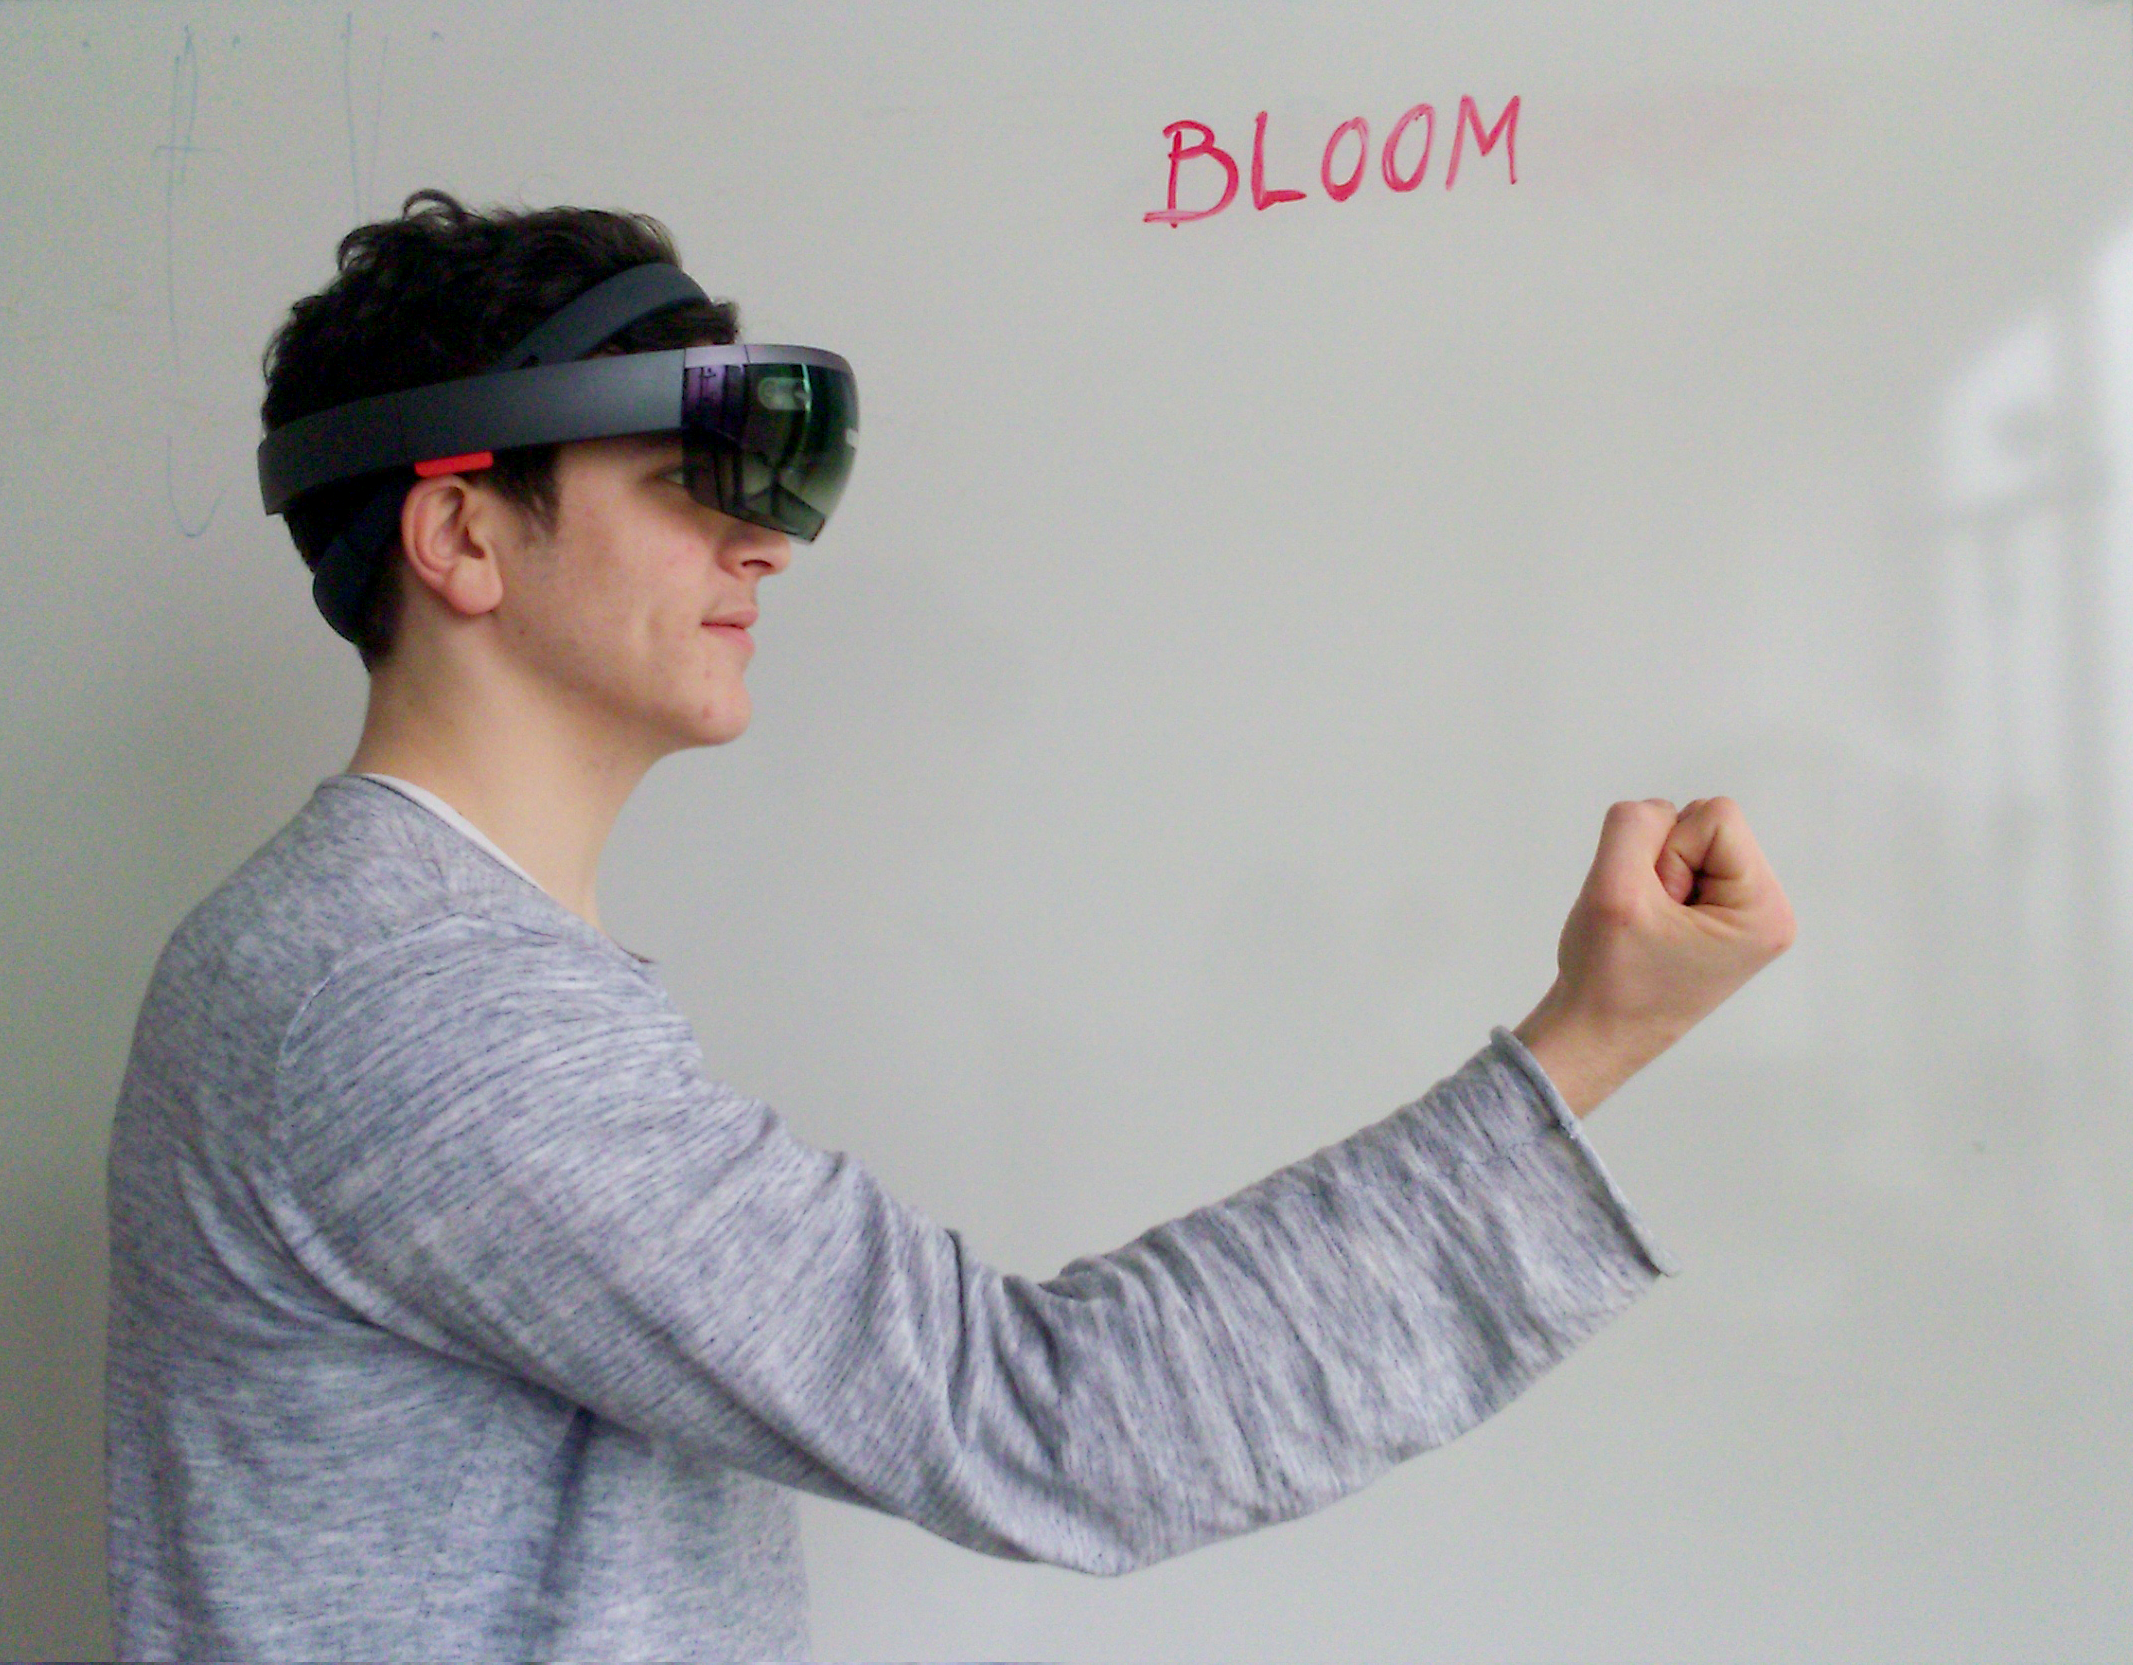
\includegraphics[width=.5\textwidth]{figuren/bloom1} &
		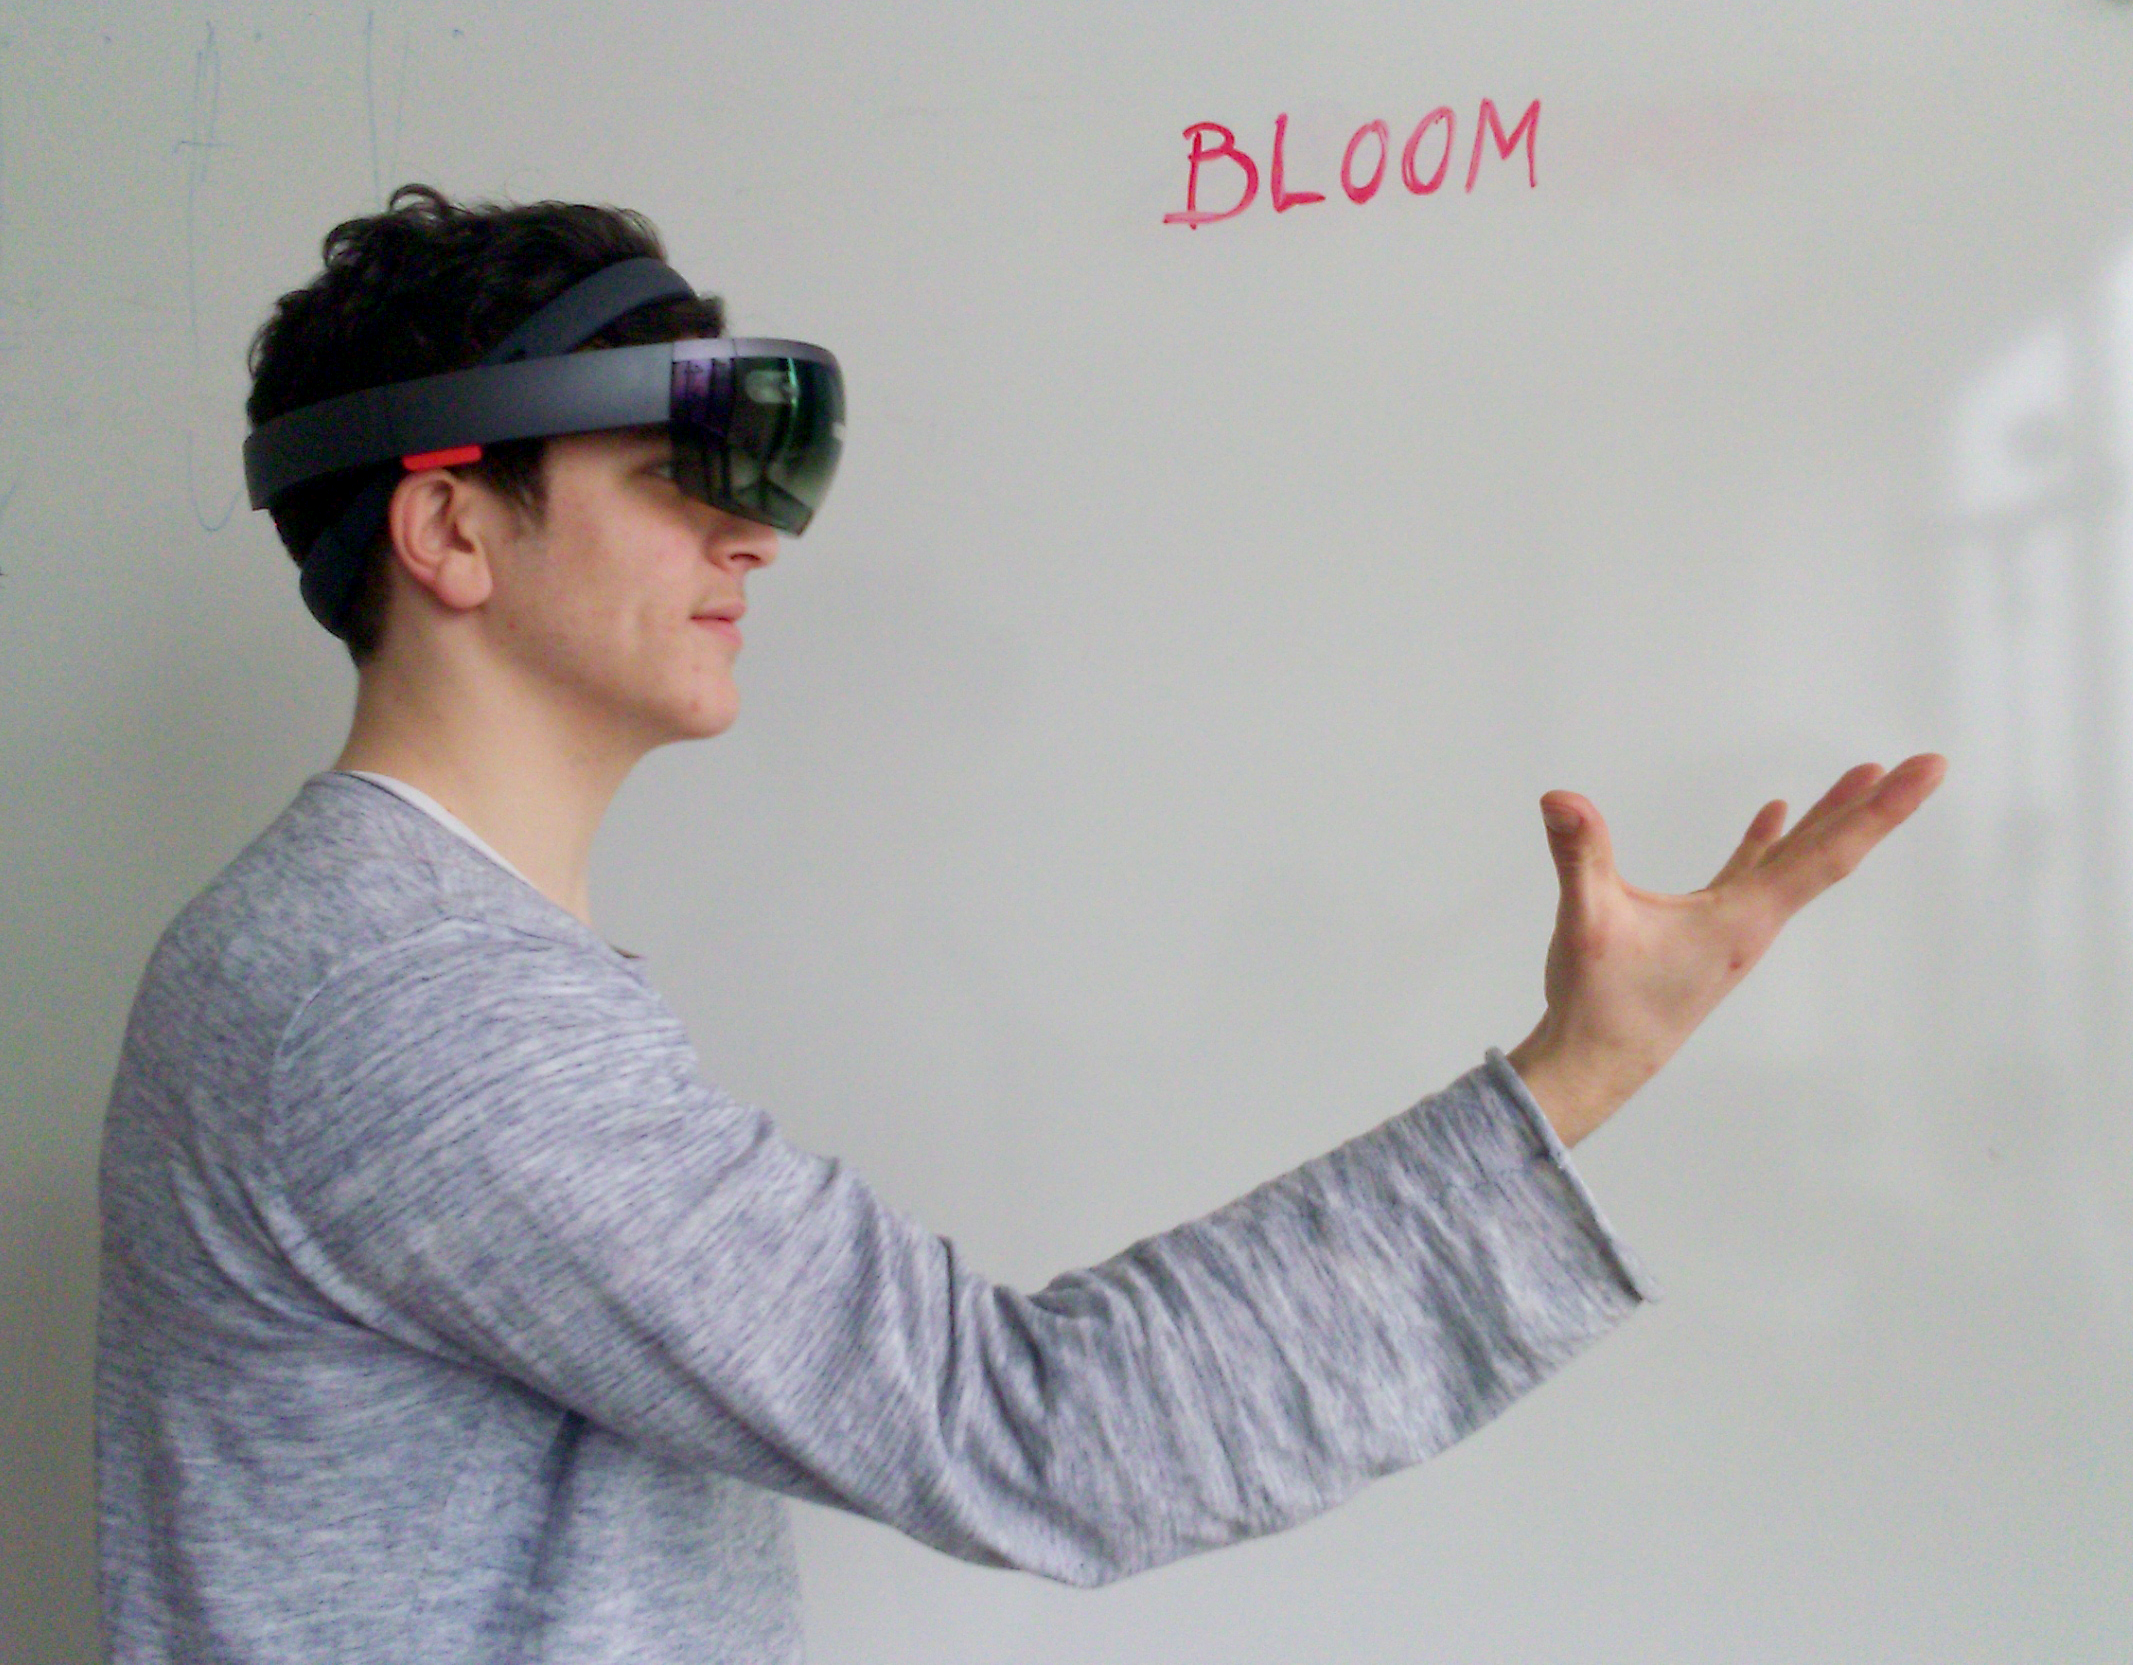
\includegraphics[width=.5\textwidth]{figuren/bloom2} \\
		(a) & (b)
	\end{tabular}
	\caption{
		\textit{Prepare Bloom Gesture (Fist)} (a), \textit{Perform Bloom Gesture} (b). Bildquelle: Eigenes Werk.
	}
	\label{fig:gesture_bloom}
\end{figure}
Die \textbf{Air-Tap}-Geste ist das Gegenstück zum klassischen Klick mit einer Maus am Computer. In Verbindung mit der \textit{Gaze}-Geste des Kopfes können somit Hologramme ausgewählt und Aktionen ausgelöst werden.\\\\Die Geste setzt sich aus einer schnellen Abfolge der \textbf{Tap-And-Hold}-Geste sowie der \textbf{Hold-And-Release}-Geste zusammen. Mit diesen lassen sich auch bekannte Manöver wie die \textit{Drag-And-Drop}-Interaktion am Computer imitieren. Beispielsweise kann man Hologramme in allen Freiheitsgraden bewegen, Bildschirminhalte verschieben (Scrollen) und andere Regler-Interaktionen, wie \textit{Zoomen} bedienen. Abbildung \ref{fig:scroll} zeigt, wie die Kombination aus diesen Gesten zusammen mit einer Translation der Hand auf der X-Achse und Y-Achse zum Scrollen verwendet werden kann.
\begin{figure}[H]
	\centering\small
	\setlength{\tabcolsep}{0mm}% alle Spaltenränder auf 0mm
	\begin{tabular}{c c} % mittlerer Abstand = 12mm
	  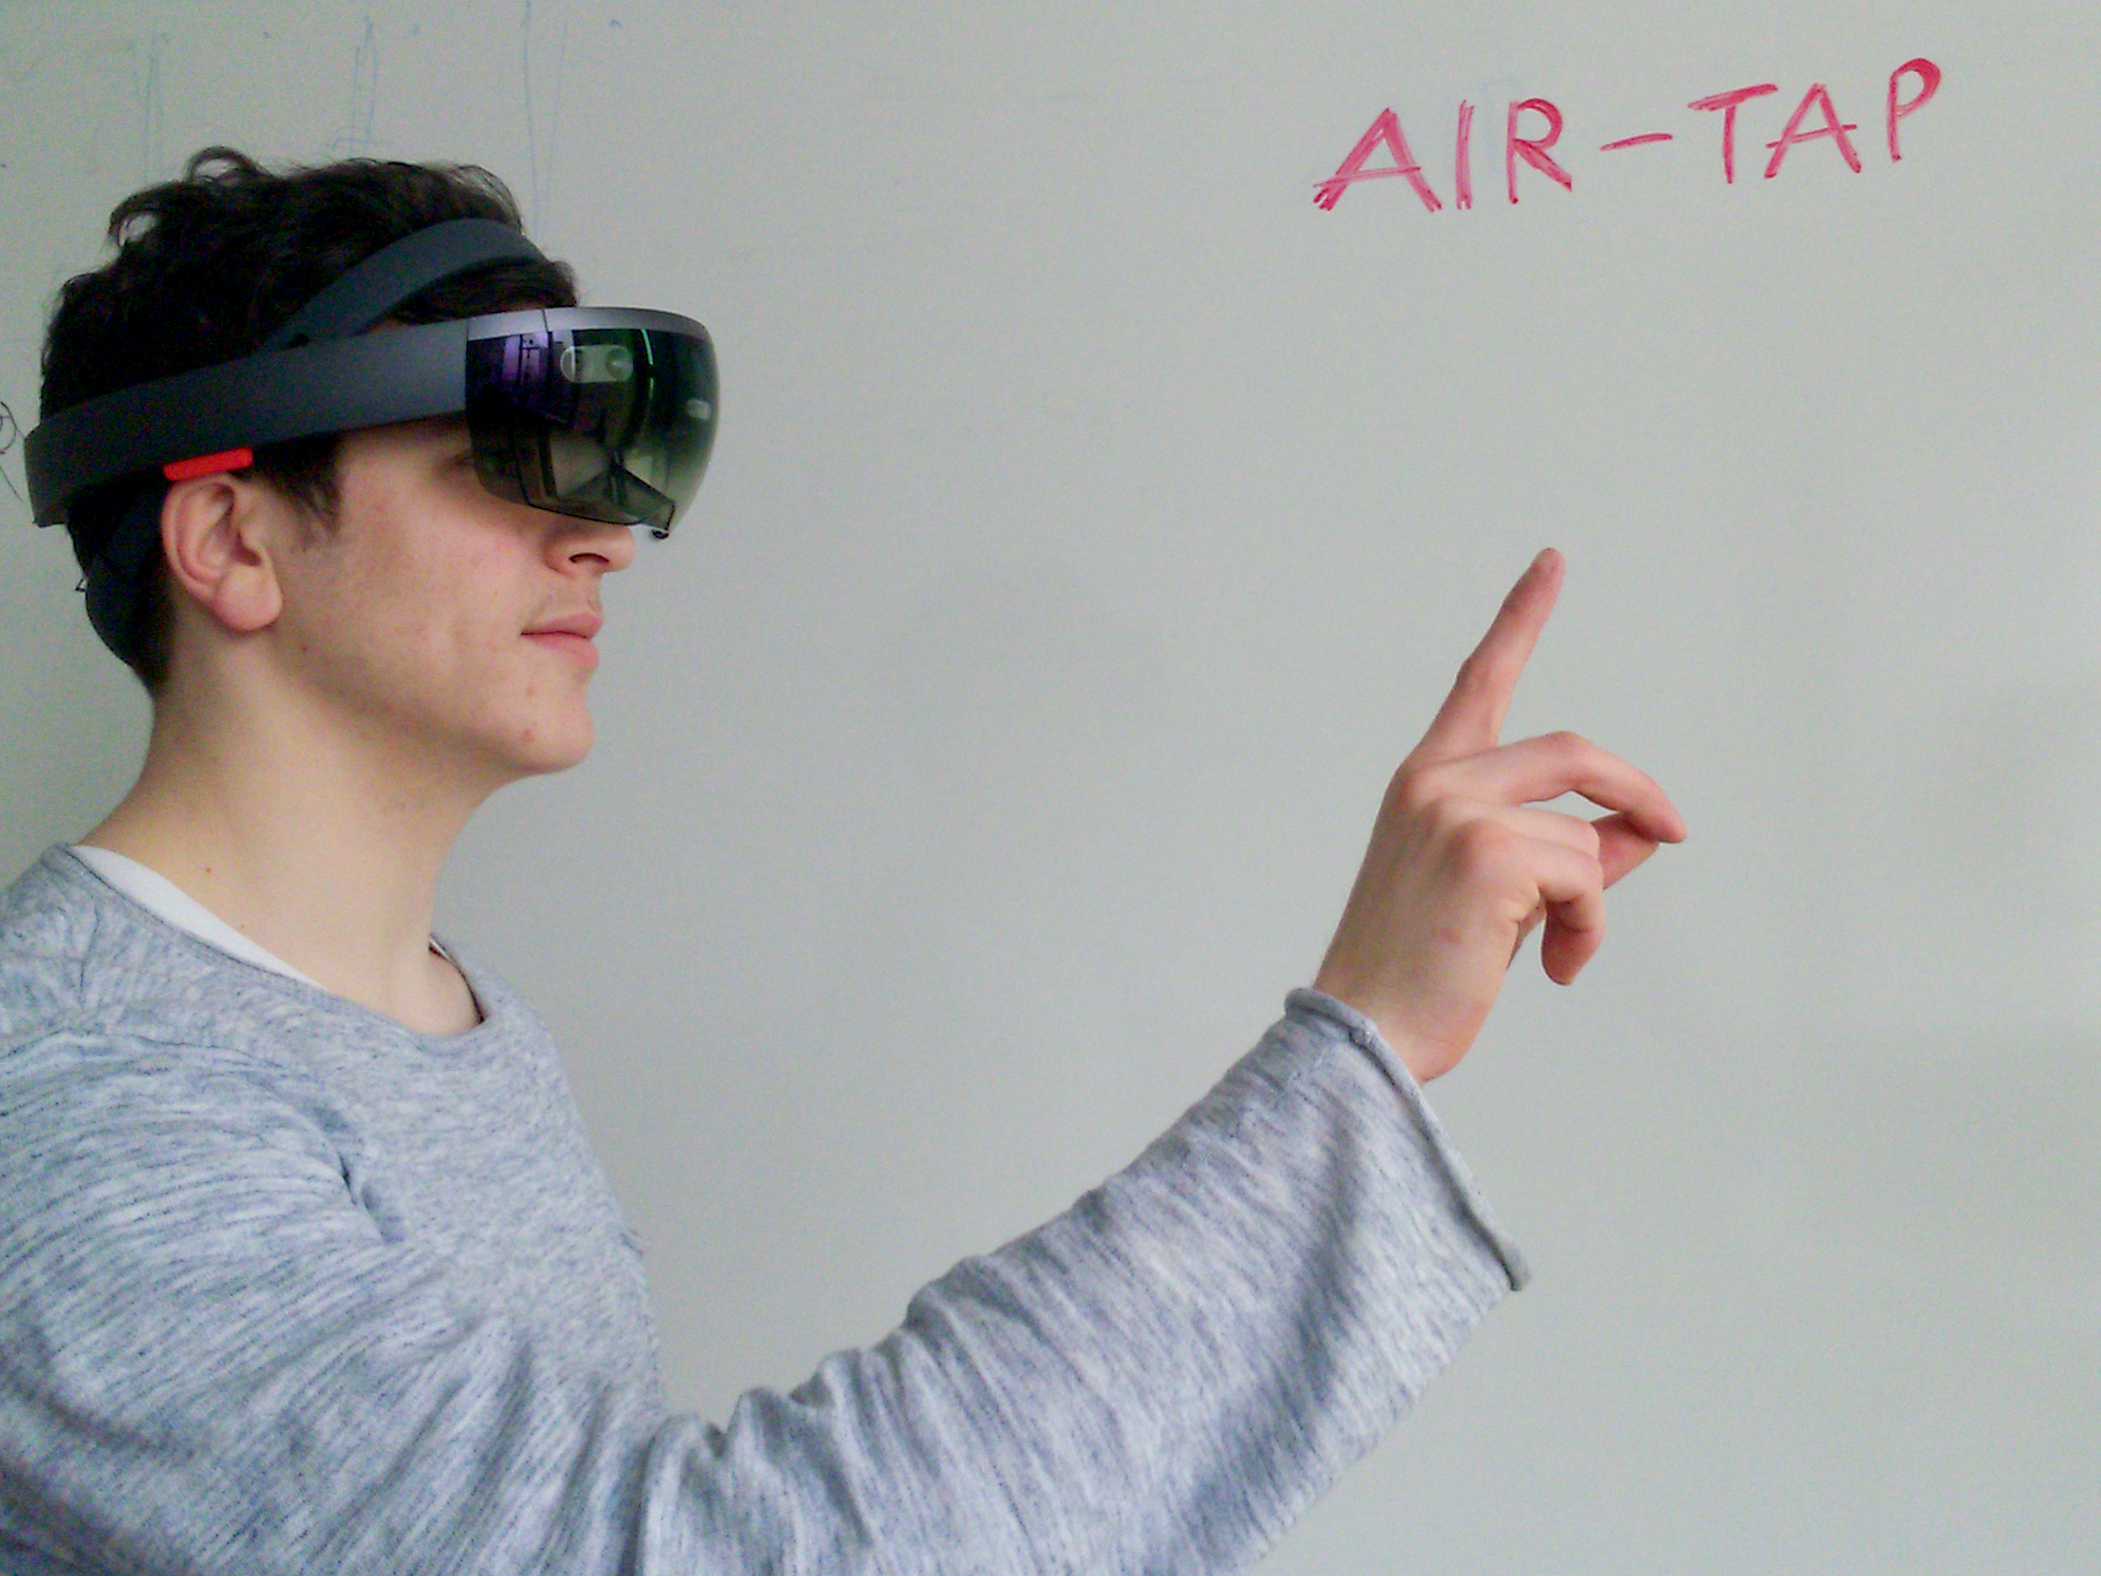
\includegraphics[width=.45\textwidth]{figuren/air_tap1} &
	  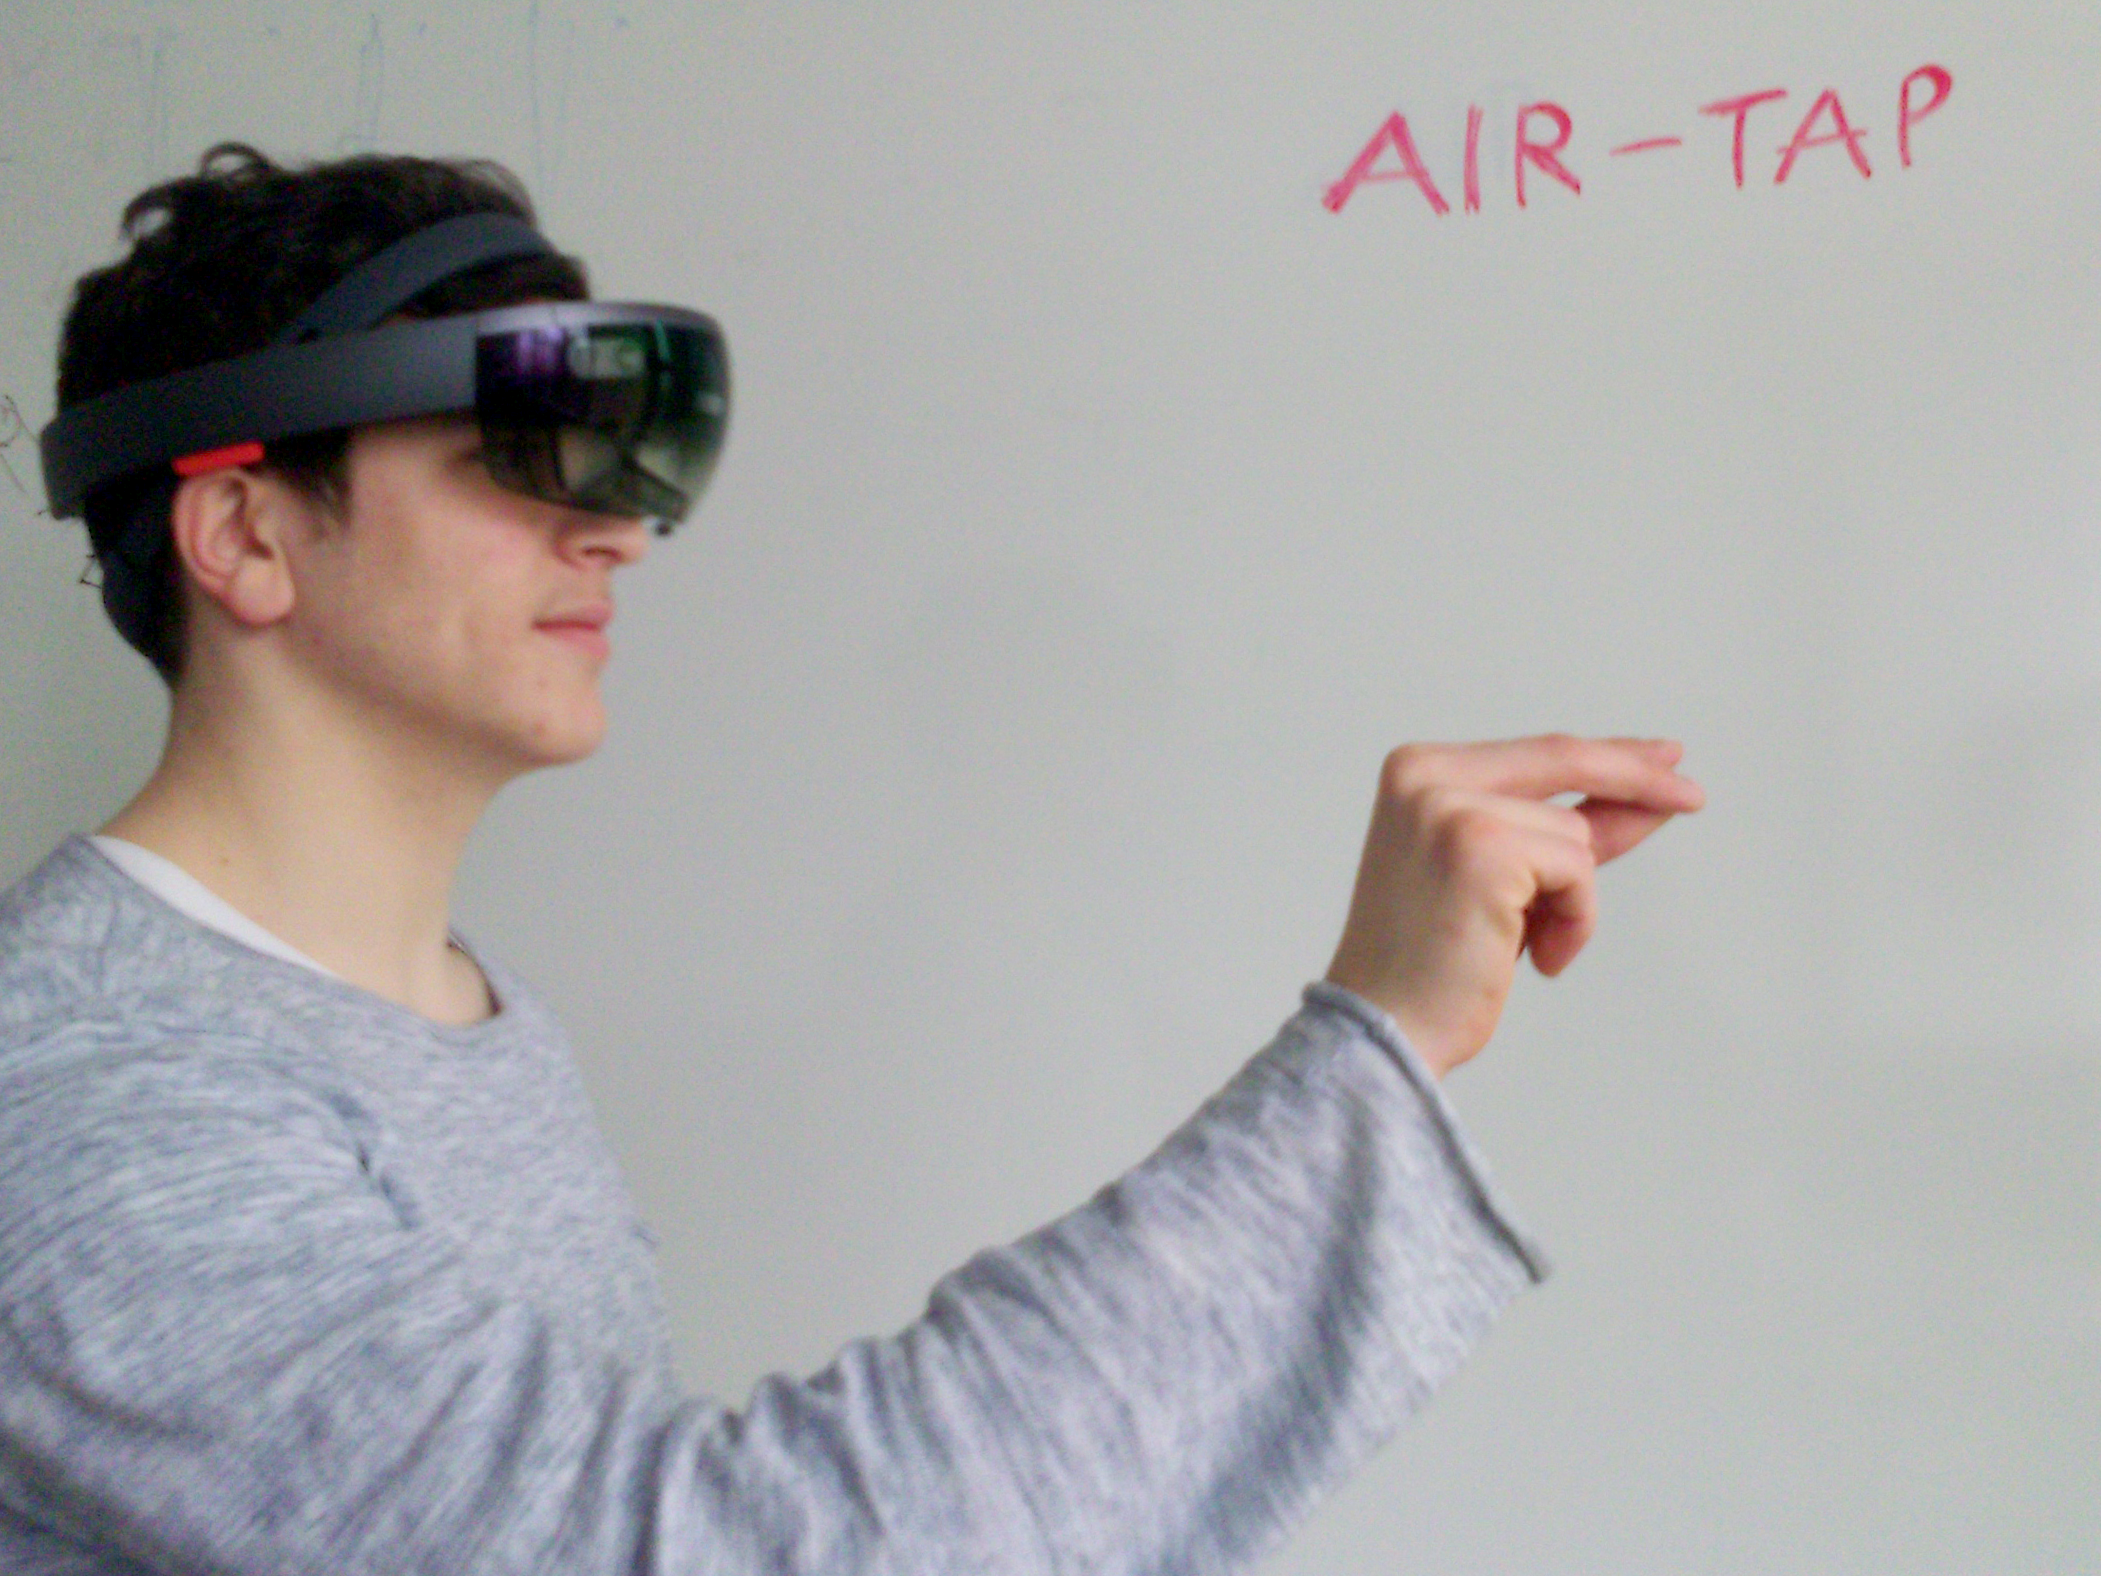
\includegraphics[width=.45\textwidth]{figuren/air_tap2} \\
	  (a) & (b) \\
	  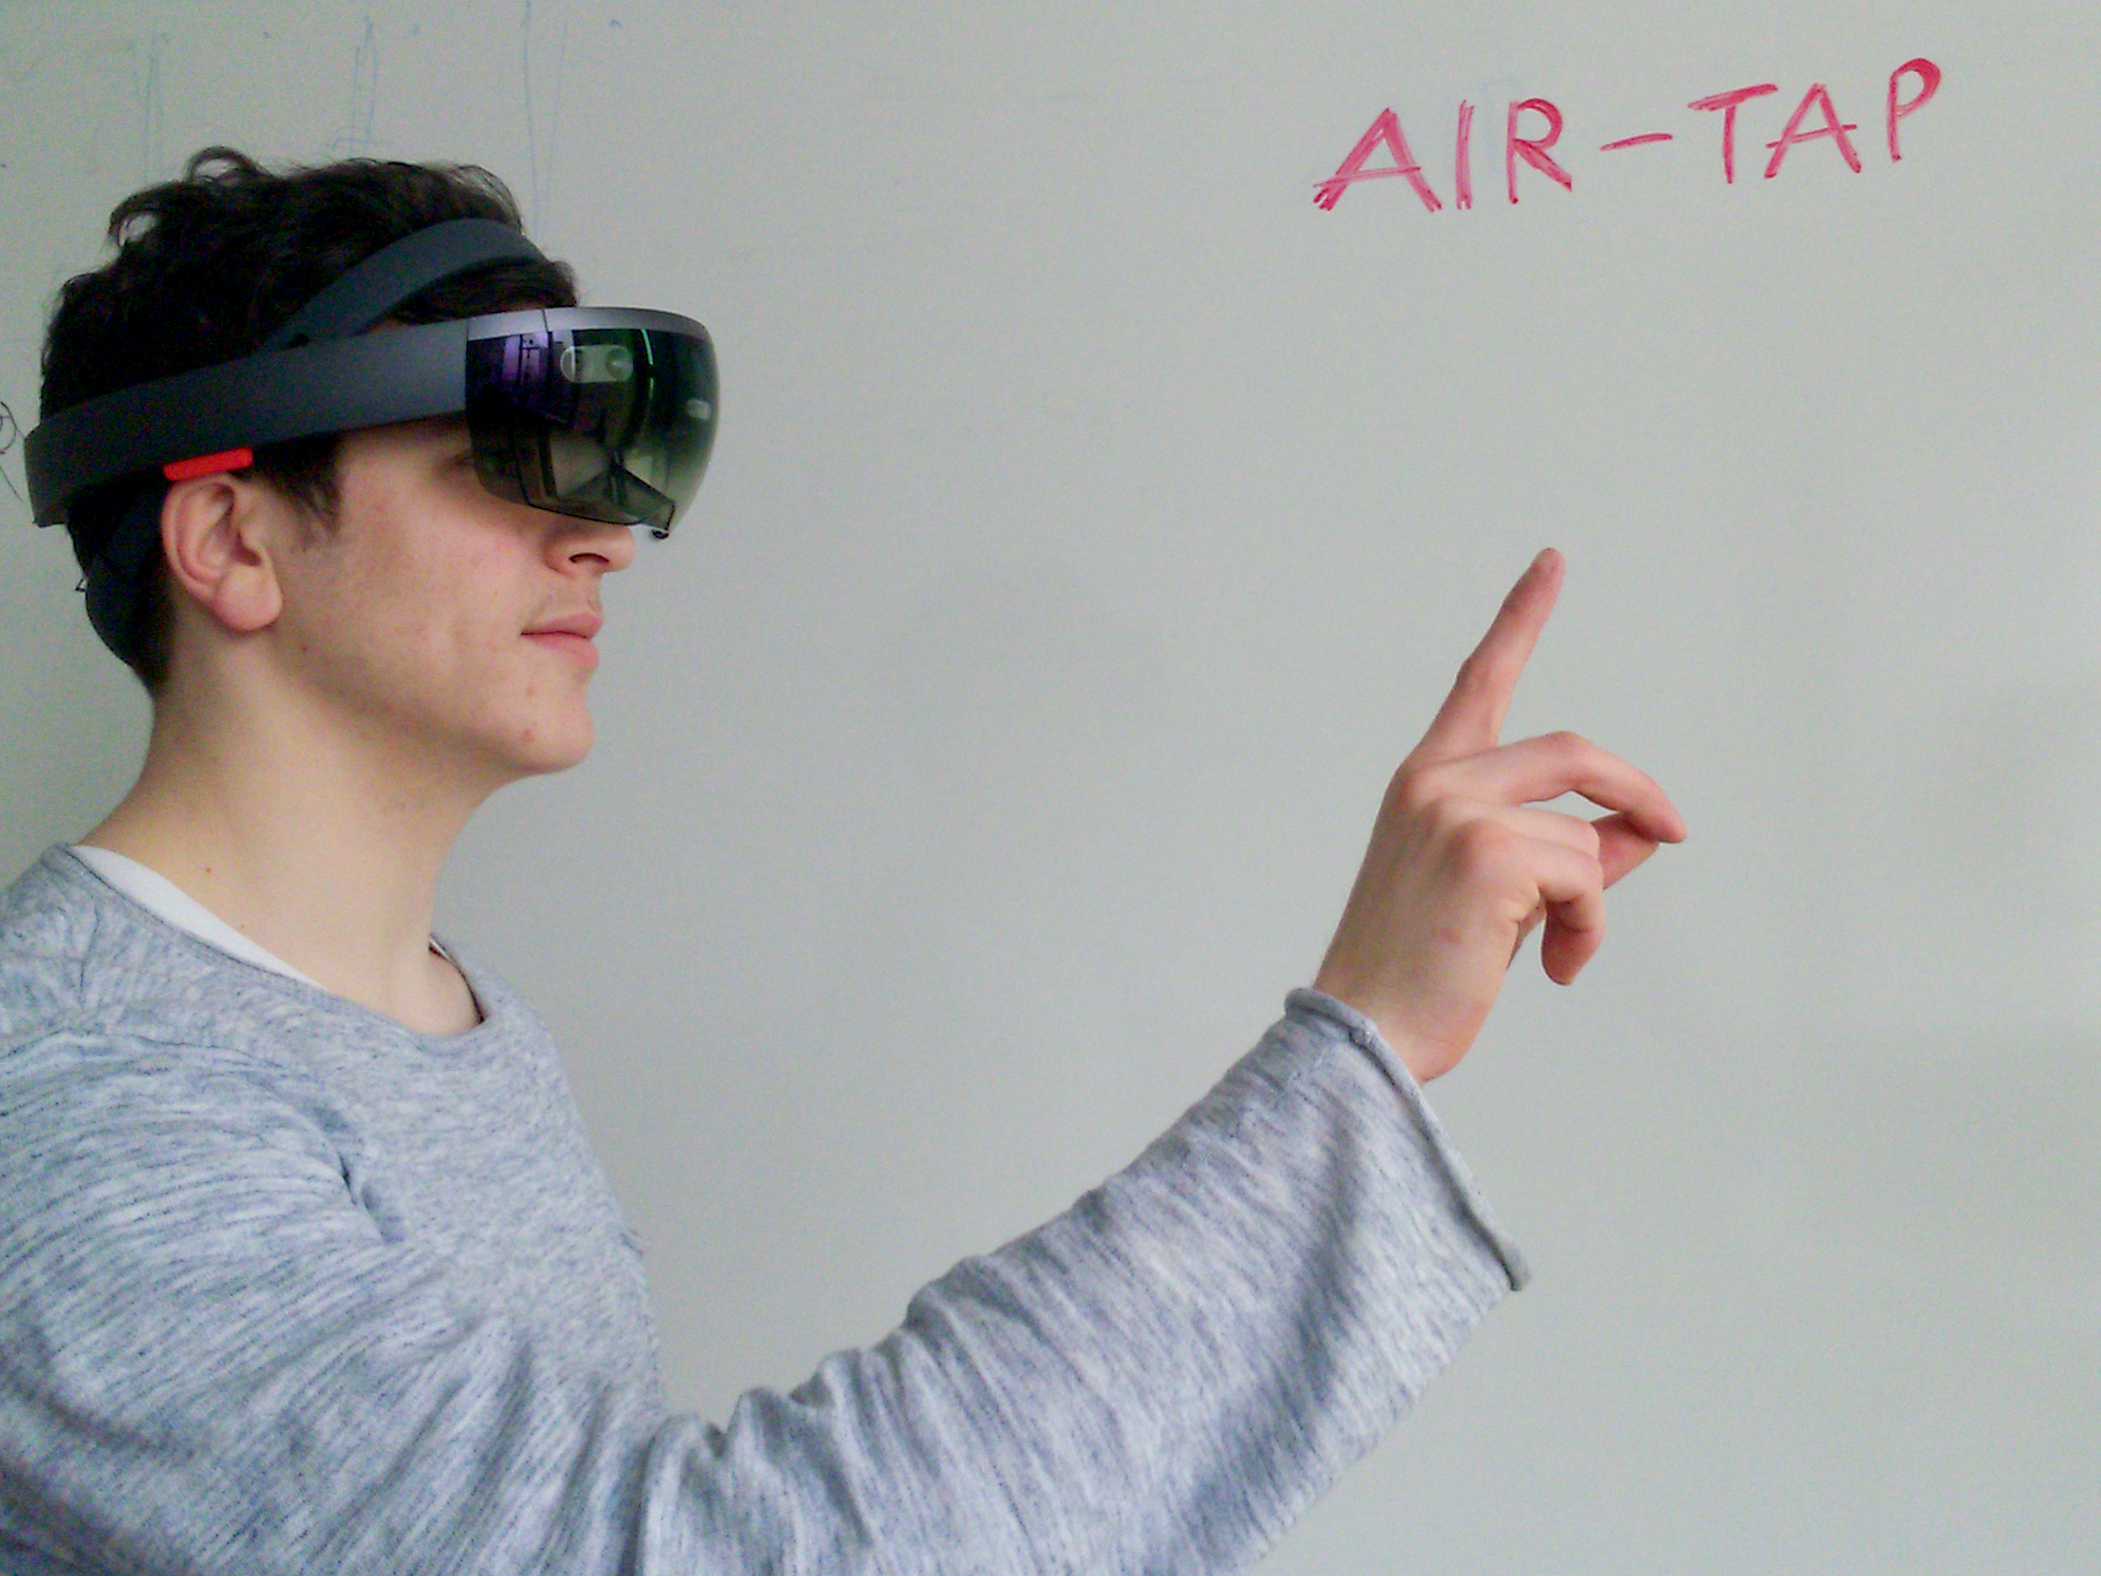
\includegraphics[width=.45\textwidth]{figuren/air_tap1} \\
	  (c)
	\end{tabular}
	%
	\caption{Die \textit{Air-Tap}-Geste. Initiiert mit der \textit{Gesture-Ready}-Geste (a), ausgeführt mit dem \textit{Tap} selbst (b) und Endposition erneute \textit{Gesture-Ready}-Geste (c). Bildquelle: Eigenes Werk.
	}
	\label{fig:gesture_air_tap}
\end{figure}
\begin{figure}[H]
	\centering
	\includegraphics[width=1.0\textwidth]{figuren/scroll}
	\caption{\textit{Scroll}-Geste in X- und Z-Richtung (\textit{Tap-And-Hold + Translation}). Bildquelle: Eigenes Werk.}
	\label{fig:scroll}
\end{figure}
\paragraph*{Voice-Commands} Die Spracherkennung der \textit{HoloLens} ist eine Interaktionsform zusätzlich zur Gesteninteraktion. In Menüs der \textit{HoloLens} sind alle interaktiven Schaltflächen auch mit Sprachkommandos aktivierbar. Dies trägt zur Barrierefreiheit bei und ist bei einer Spracherkennung mit einer Wort-zu-Fehlerrate von 5,9 Prozent durchaus als ein verlässliches Werkzeug anzusehen.\footnote{ Vgl. Xiong / Droppo / Huang / et al, o.S., 2016.}
\begin{figure}[H]
	\centering
	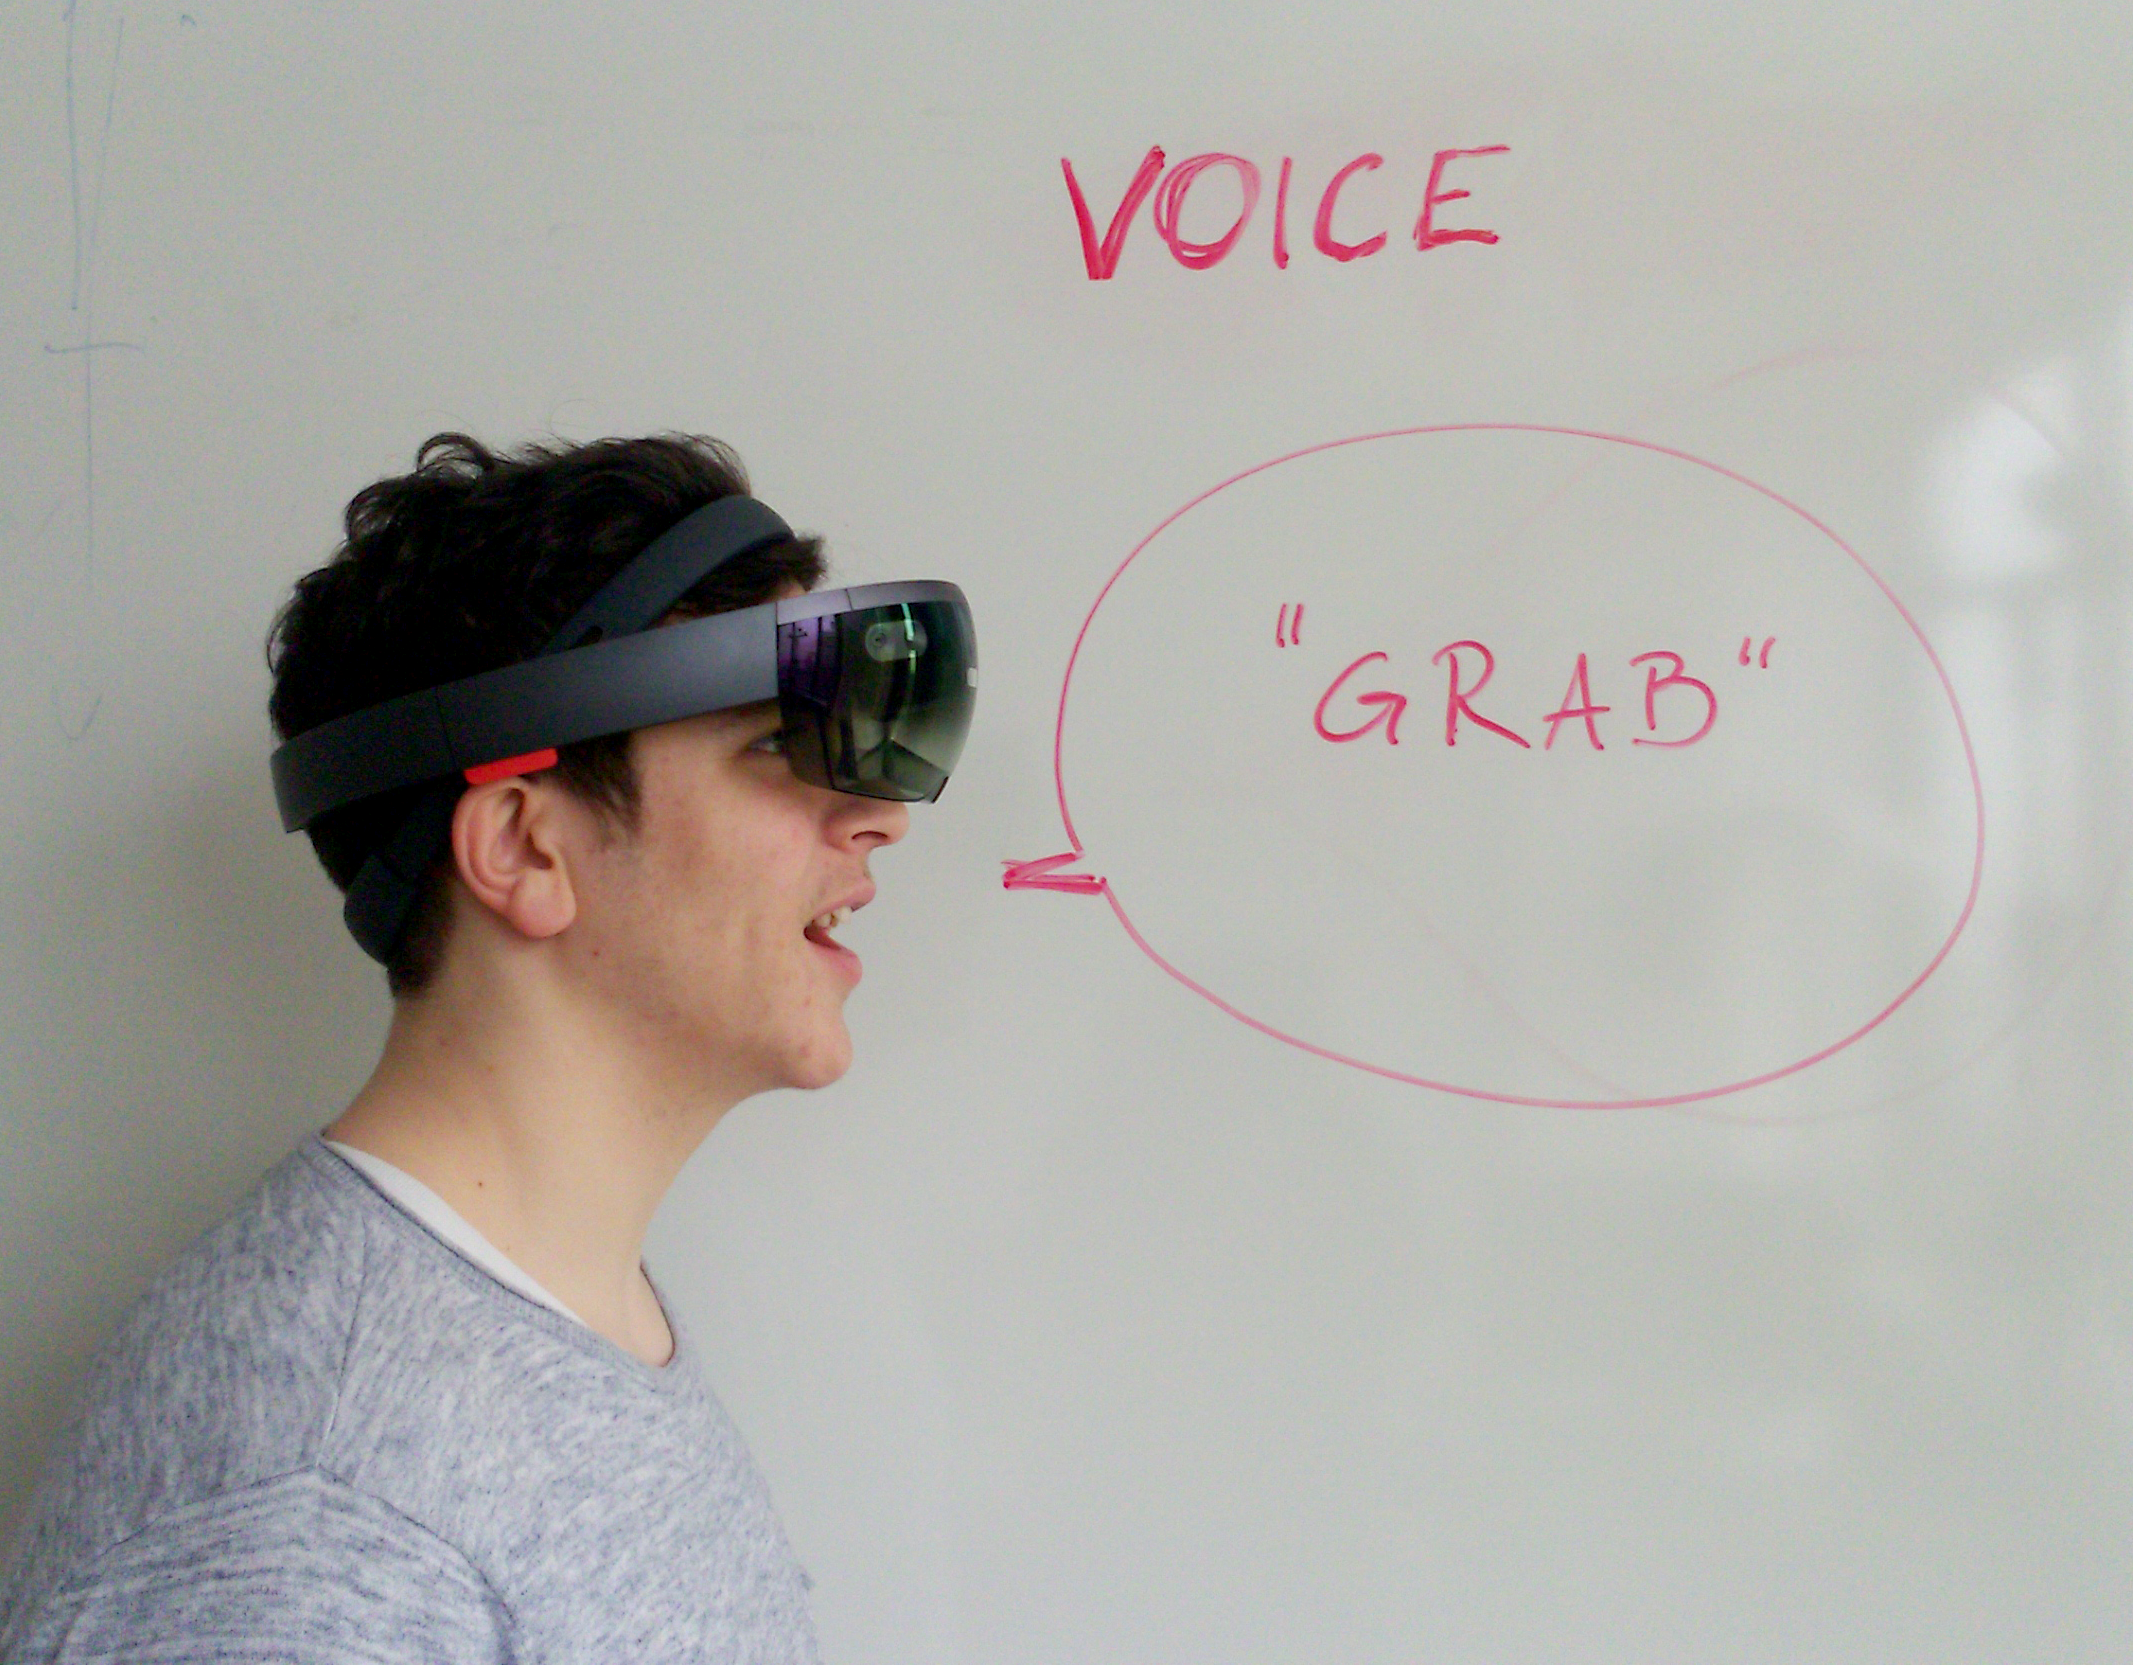
\includegraphics[width=1.0\textwidth]{figuren/voice}
	\caption{\textit{Voice-Command}: Am Beispiel \frqq Grab\flqq. Bildquelle: Eigenes Werk.}
	\label{fig:voice_command}
\end{figure}
Die Gesten- und Sprachinteraktion sind den HCI-Kriterien der ISO 9241-110\footnote{DIN 9241-110, Hrsg., o.S., 2008.} für Soft- und Hardwaresysteme nachempfunden. Sie tragen abgekürzt den Namen \frqq ASSEFIL\flqq-Kriterien:\begin{enumerate}
	\item Aufgabenangemessenheit:\\\frqq Ein Dialog ist aufgabenangemessen, wenn er den Benutzer unterstützt, seine Arbeitsaufgabe effektiv und effizient zu erledigen.\flqq
	\item Selbstbeschreibungsfähigkeit:\\\frqq Wenn eine Eingabe verlangt wird, sollte das Dialogsystem dem Benutzer Informationen über die zu erwartete Eingabe geben.\flqq
	\item Steuerbarkeit:\\\frqq Ein Dialog steuerbar, wenn der Benutzer in der Lage ist, den Dialogablauf zu starten sowie seine Richtung und Geschwindigkeit zu beeinflussen, bis das Ziel erreicht ist\flqq
	\item Erwartungskonformität:\\\frqq Ein Dialog ist erwartungskonform, wenn er konsistent ist und den Merkmalen des Benutzers entspricht, zum Beispiel seinen Kenntnissen aus dem Arbeitsgebiet und seinen Erfahrungen sowie den allgemein anerkannten Konventionen.\flqq
	\item Fehlertoleranz:\\\frqq Ein Dialog ist fehlertolerant, wenn das beabsichtigte Arbeitsergebnis trotz erkennbarer Fehleingaben entweder mit keinem oder mit minimalem Korrekturaufwand seitens des Benutzers erreicht werden kann.\flqq
	\item Individualisierbarkeit:\\\frqq Ein Dialog ist individualisierbar, wenn Benutzer die Mensch-System-Interaktion und die Darstellung von Informationen ändern können, um dise an ihre individuellen Fähigkeiten und Bedürfnisse anzupassen.\flqq
	\item Lernförderlichkeit:\\\frqq Ein Dialog ist lernförderlich, wenn er den Benutzer beim Erlernen der Nutzung des interaktiven Systems unterstützt und anleitet.\flqq
\end{enumerate}
Im nächsten Kapitel wird, mit den im Kapitel~\ref{chapter:Grundlagen} vorgestellten Technologien und Interaktionen, das Konzept für die prototypische Implementierung vorgestellt.
\newpage